\documentclass[12pt, orivec]{article}
\usepackage{amsmath}
\usepackage{amssymb}    % for \rightsquigarrow
\usepackage{wasysym}	% for frown face
\usepackage[most]{tcolorbox}
\usepackage{ulem}
\usepackage{tikz-cd}		% commutative diagrams
\usepackage{tikz}
\usepackage{amsthm}
\usepackage{enumitem}	% for \itemize custom labels
\usepackage{turnstile}	% longer turnstiles
\usepackage[sf,bf,big,raggedright,compact]{titlesec}	% change section color to blue
\usepackage[backend=biber,bibstyle=authoryear,citestyle=authoryearbrack]{biblatex}
\bibliography{../AGI-book}

\newtheorem{theorem}{Theorem}

\ifdefined\chinchin
\usepackage[CJKspace]{xeCJK}
\setCJKmainfont[BoldFont=SimHei,ItalicFont=AR PL KaitiM GB]{SimSun}
\newcommand{\cc}[2]{#1}
\else
\newcommand{\cc}[2]{#2}
\fi

\setcounter{secnumdepth}{0}		% no section numbers

\titleformat{\section}[hang]{\bfseries\Large\color{blue}}{\thesection \hspace{10pt}}{0pt}{}
\titleformat{\subsection}[hang]{\bfseries\large\color{blue}}{\thesubsection \hspace{5pt}}{0pt}{}

\newcommand{\book}[1]{$\NewSym[0.4]{../book-icon.png} \quad$ \parbox{0.9\textwidth}{\footnotesize #1}}
\newcommand{\code}[1]{{\footnotesize{\ttfamily #1}}}
\newcommand{\tab}{\hspace*{2cm}}
\newcommand{\powerset}{\raisebox{.15\baselineskip}{\Large\ensuremath{\wp}}}
\newcommand{\Chi}{\raisebox{2.5pt}{$\chi$}}
\newcommand*\KB{\vcenter{\hbox{\includegraphics{../KB-symbol.png}}}}
\newcommand*\NewSym[2][0.5]{\vcenter{\hbox{\includegraphics[scale=#1]{#2}}}}
\newcommand*\sigmoid{\vcenter{\hbox{
\includegraphics{sigmoid.png}}}}
\newcommand{\smbox}[1]{\boxed{\footnotesize{\mbox{#1}}}}

\newcommand{\tikzmark}[1]{\tikz[overlay,remember picture] \node (#1) {};}

\newcommand{\Dfrac}[2]{%
\ooalign{%
      $\genfrac{}{}{2.9pt}0{\hphantom{#1}}{\hphantom{#2}}$\cr%
      $\color{white}\genfrac{}{}{1.5pt}0{\hphantom{#1}}{\hphantom{#2}}$\cr%
      $\color{white}\genfrac{}{}{1pt}0{\color{black}#1}{\color{black}#2}$}}

\renewcommand{\thefootnote}{\fnsymbol{footnote}}
\interfootnotelinepenalty=10000

\title{\cc{人工智能的知识表述}{Knowledge representation in AI}}
\author{\cc{甄景贤}{Yan King Yin} {\footnotesize general.intelligence@gmail.com}}

\begin{document}
\setlength{\parindent}{0pt}
\setlength{\parskip}{2.8ex plus0.8ex minus0.8ex}

\maketitle

\tableofcontents

\begin{abstract}
As of now (2018 August), the question of strong AI is no longer whether it is possible or not, but whether one feasible approach is better than another.  The tutorial introduces the mathematical theory of knowledge representations, and discusses 3 proposals, respectively based on:  A) genetic algorithms;  B) neural networks + graphs;  C) geometric models.
\end{abstract}

\section{What is model theory?}

For example, \textbf{hyperbolic geometry} can be ``realized'' by the following \textbf{models}:
\begin{equation}
\vcenter{\hbox{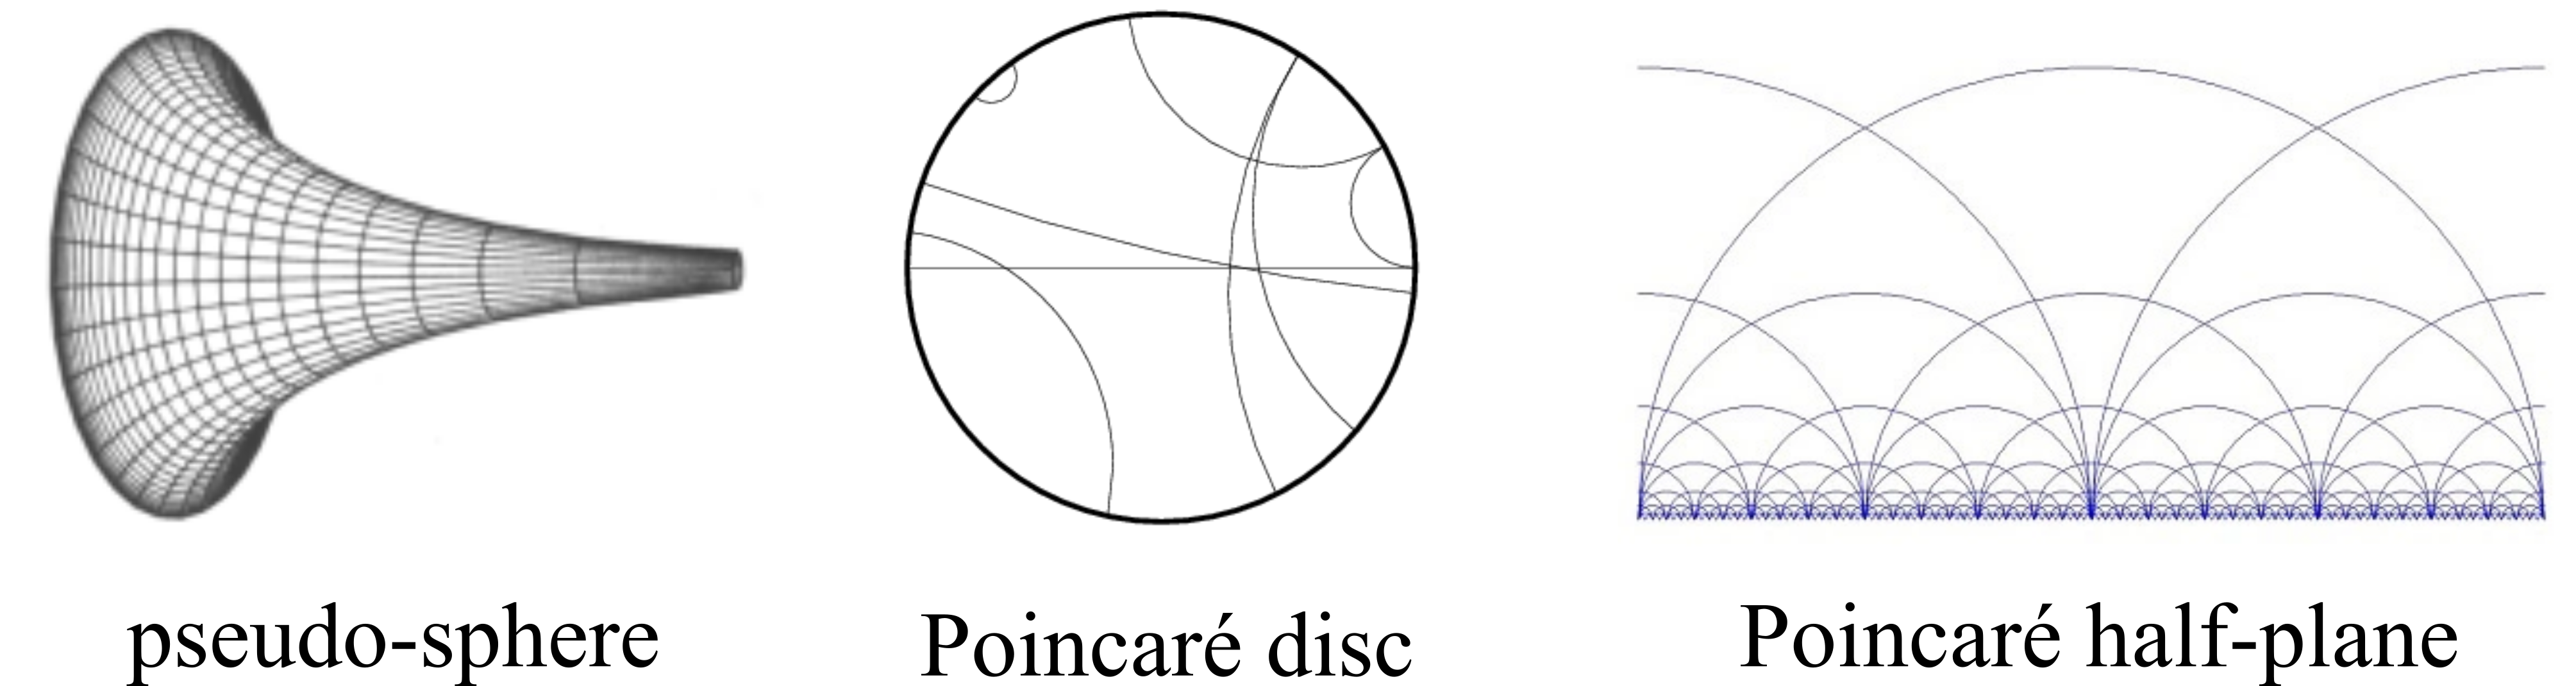
\includegraphics[scale=0.65]{hyperbolic-models.png}}} 
\end{equation}
Models are not unique, there can be many models for a theory.

In mathematical logic, \textbf{model theory} studies the \textbf{duality} between \textbf{syntax} and \textbf{models}.

The most classic example is \textbf{Stone duality}, also familiar to all of us as ``Venn diagrams'':
\begin{equation}
P \wedge Q \quad \cong \quad
\vcenter{\hbox{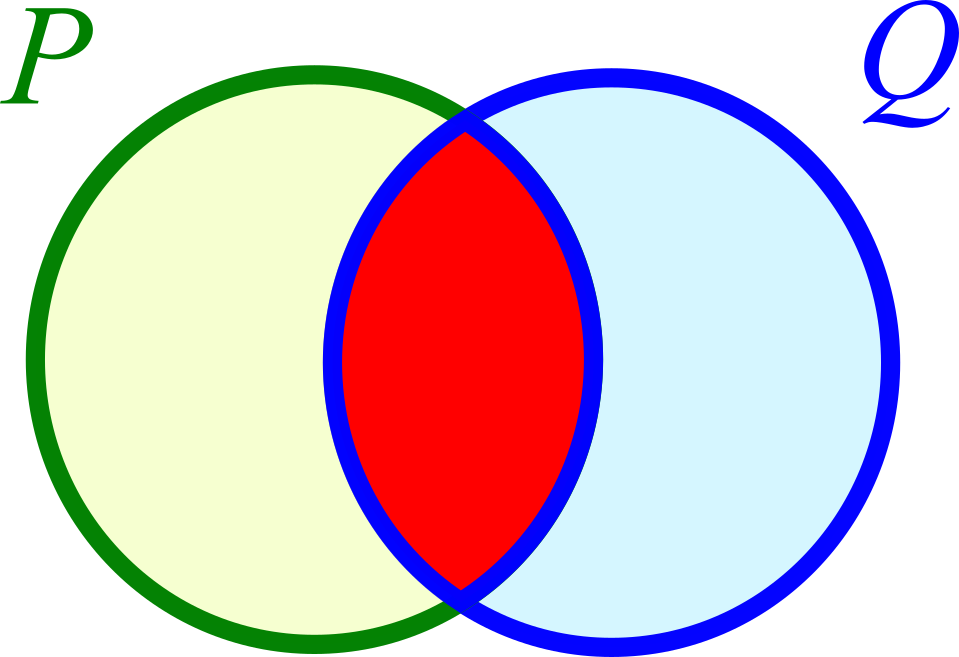
\includegraphics[scale=0.7]{Venn-diagram-0.png}}}
\end{equation}
Stone duality\footnote{Marshall Stone (1903-1989), American mathematician who contributed to real analysis, functional analysis, topology and the study of Boolean algebras.} 
refers to the duality between \textbf{Boolean algebras} and \textbf{topological spaces}.

Boolean algebra is the same as \textbf{propositional logic}, which concerns only with the truth and falsehood of propositions.  For example, P = \textit{``It is raining in New York''}, but we cannot ``access'' the internal constituents of the propositioon, such as \textit{``rain''} and \textit{``New York''}.  The critical obstruction to strong AI is the \textbf{lifting} from propositional to first-order logic.

First-order logic can be modeled by \textbf{sets} and their \textbf{elements}.  For example \\
$\mbox{John} \in \mbox{Male}, \quad \mbox{John, Mary} \in \mbox{Mathematician}$: 
\begin{equation}
\vcenter{\hbox{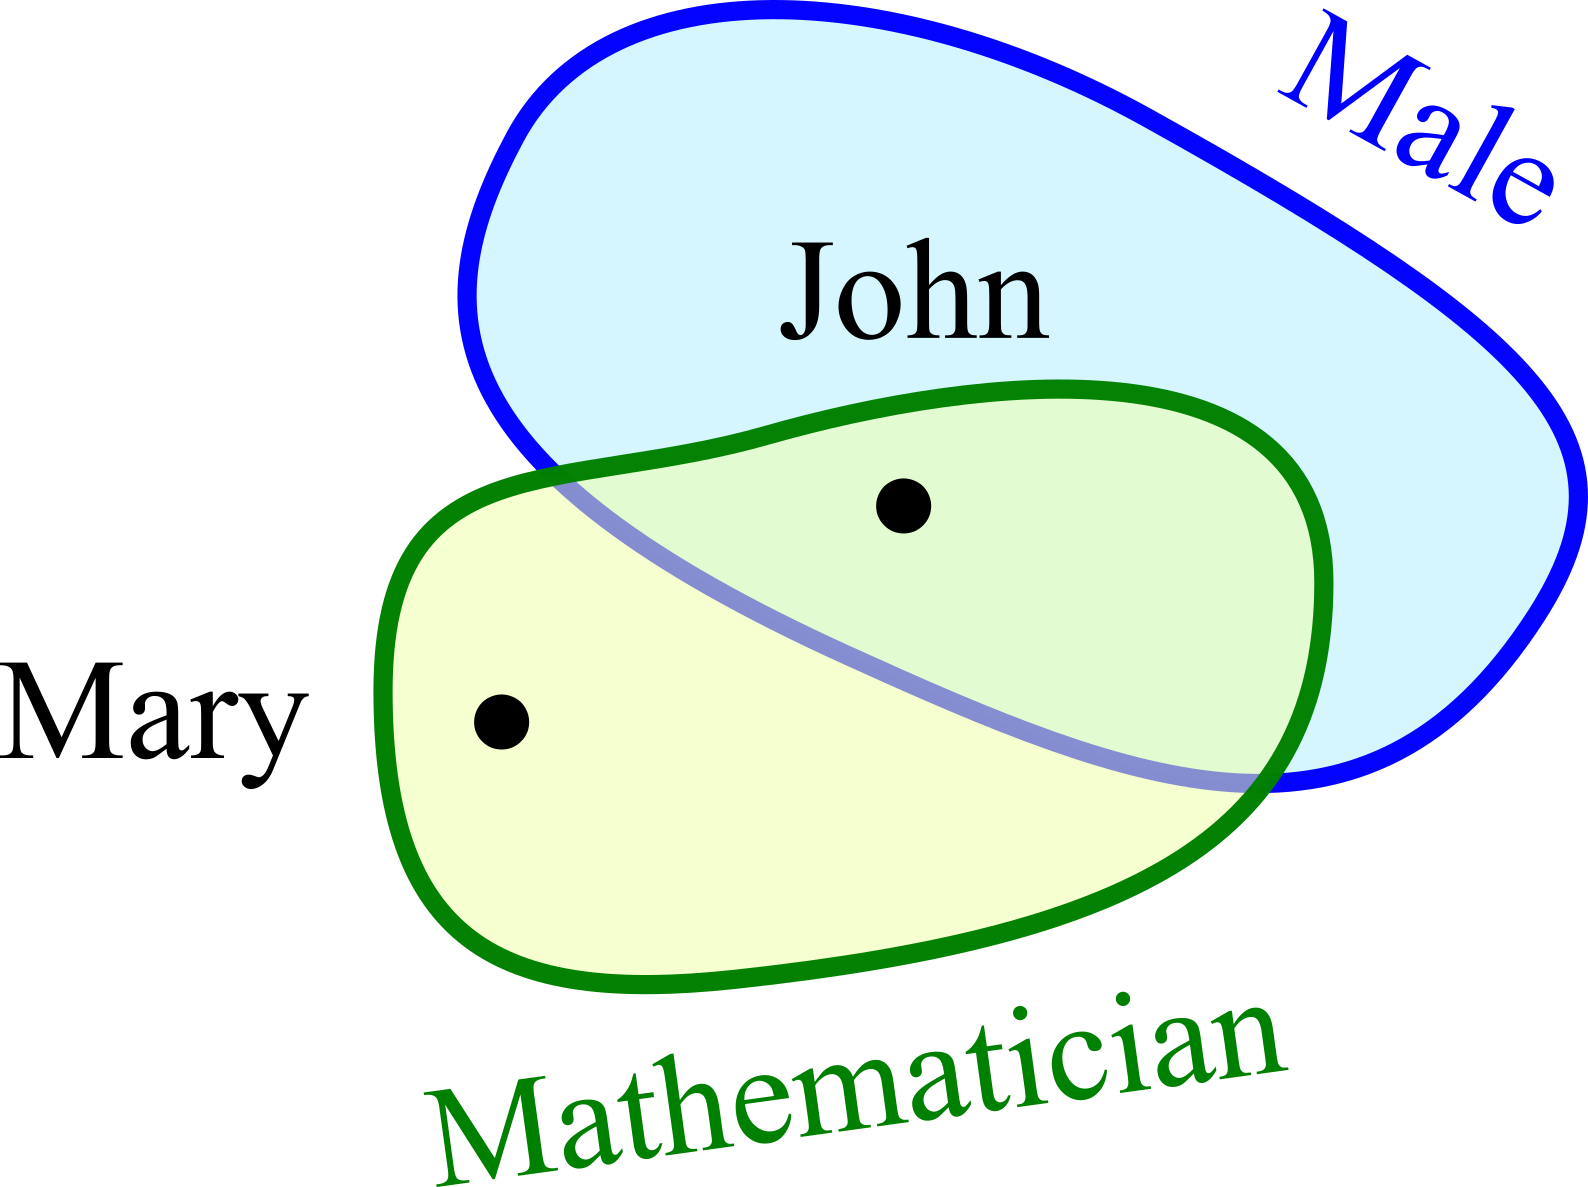
\includegraphics[scale=0.6]{FOL-model-1.png}}} 
\end{equation}
Whereas \textbf{relations} between first-order \textbf{objects} in a domain $D$ are represented by \textbf{subsets} of the Cartesian product $D \times D$, eg:
\begin{equation}
\vcenter{\hbox{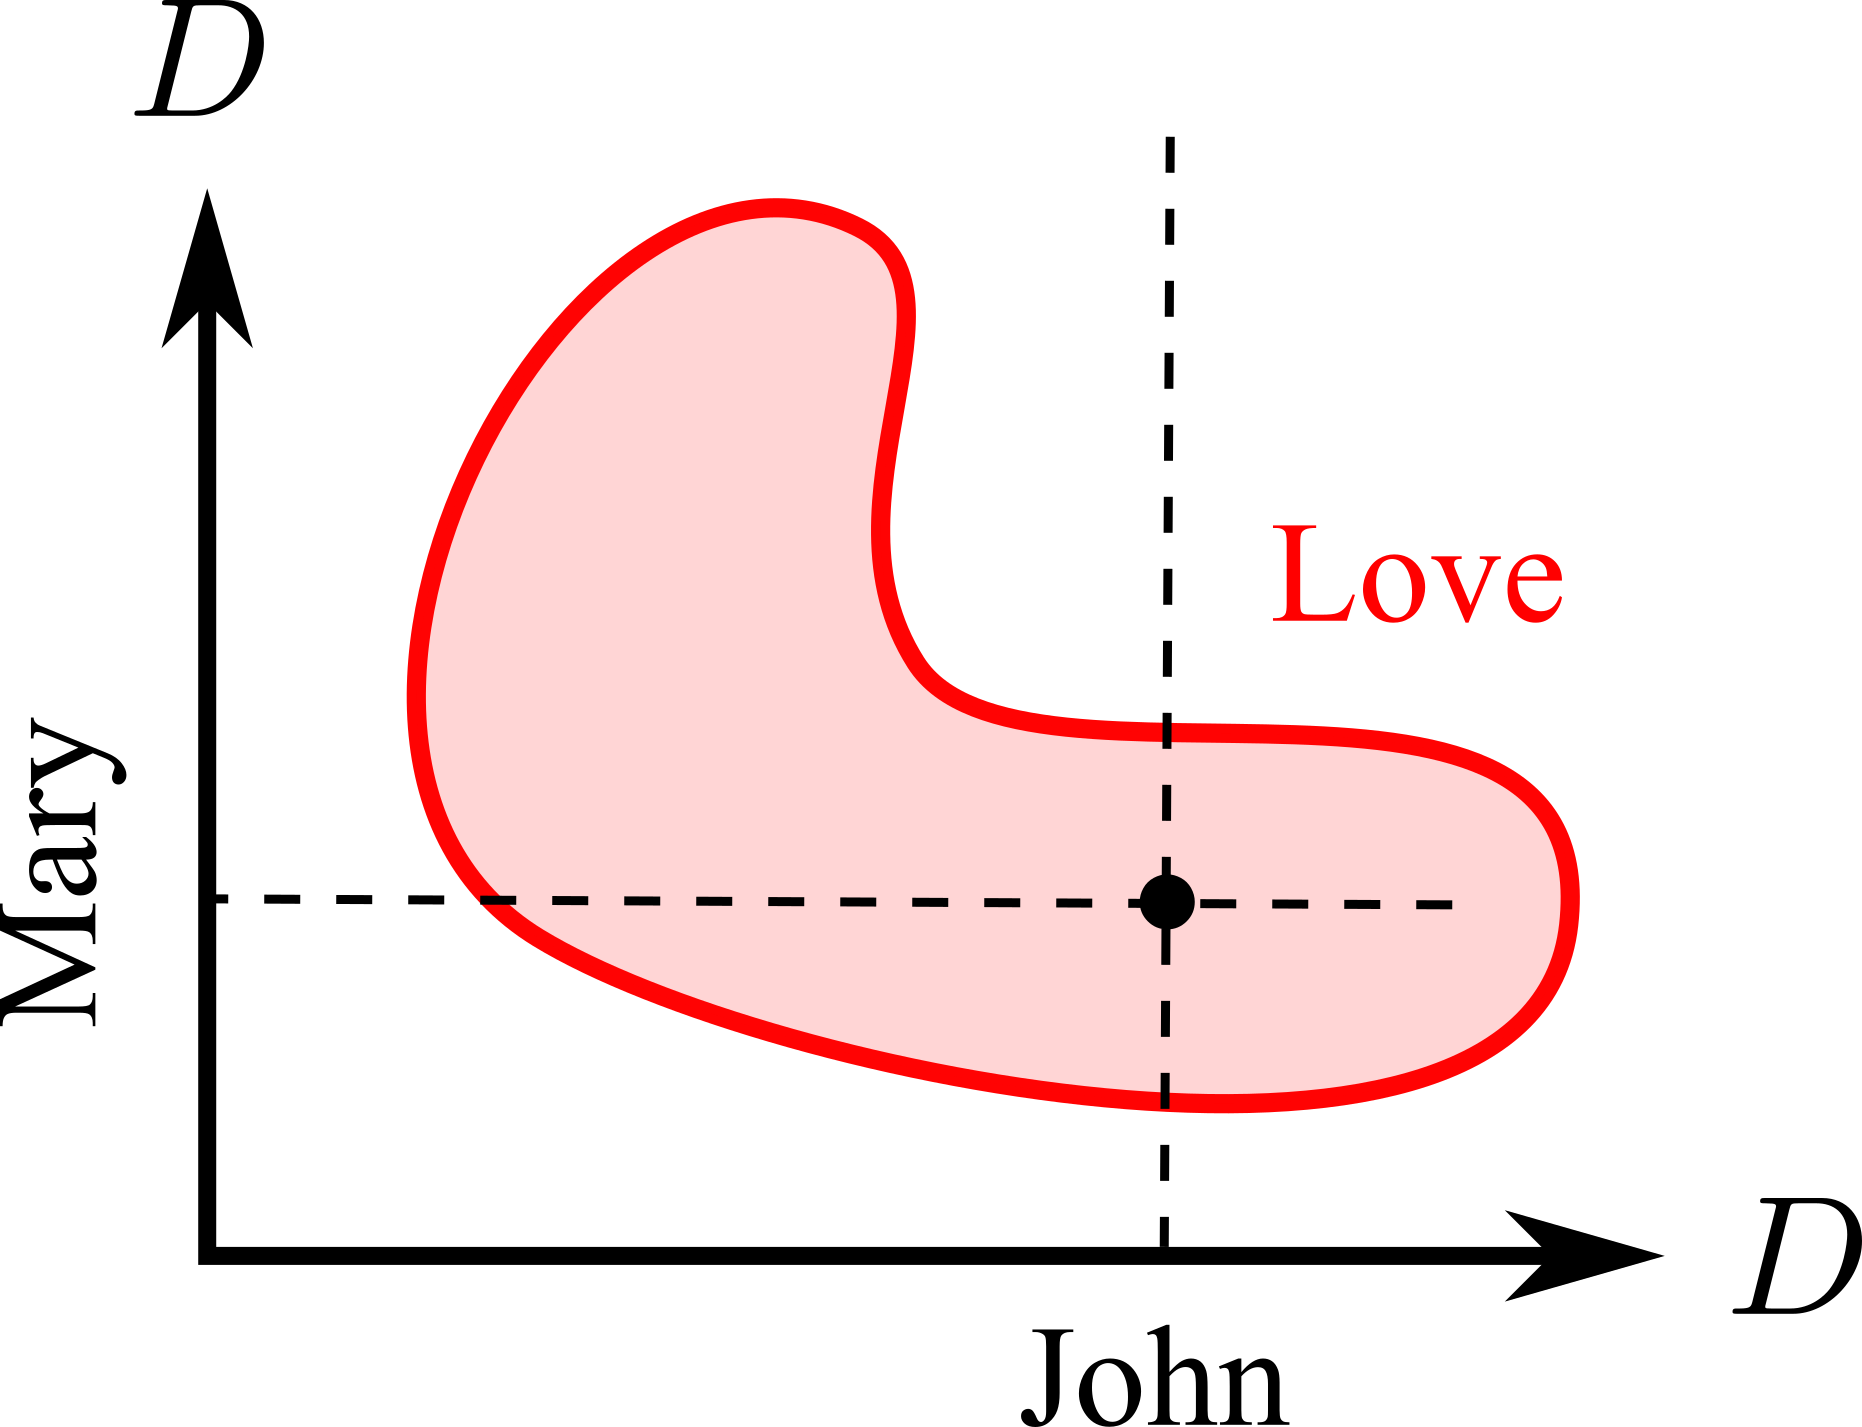
\includegraphics[scale=0.5]{FOL-model-2.png}}} 
\end{equation}

What the fuck's wrong with this line?

For computer science people, 

you may be more familiar with \textbf{relation graphs}

or \textbf{knowledge graphs} such as this one:

What the fuck's wrong with this line?

\begin{equation}
\vcenter{\hbox{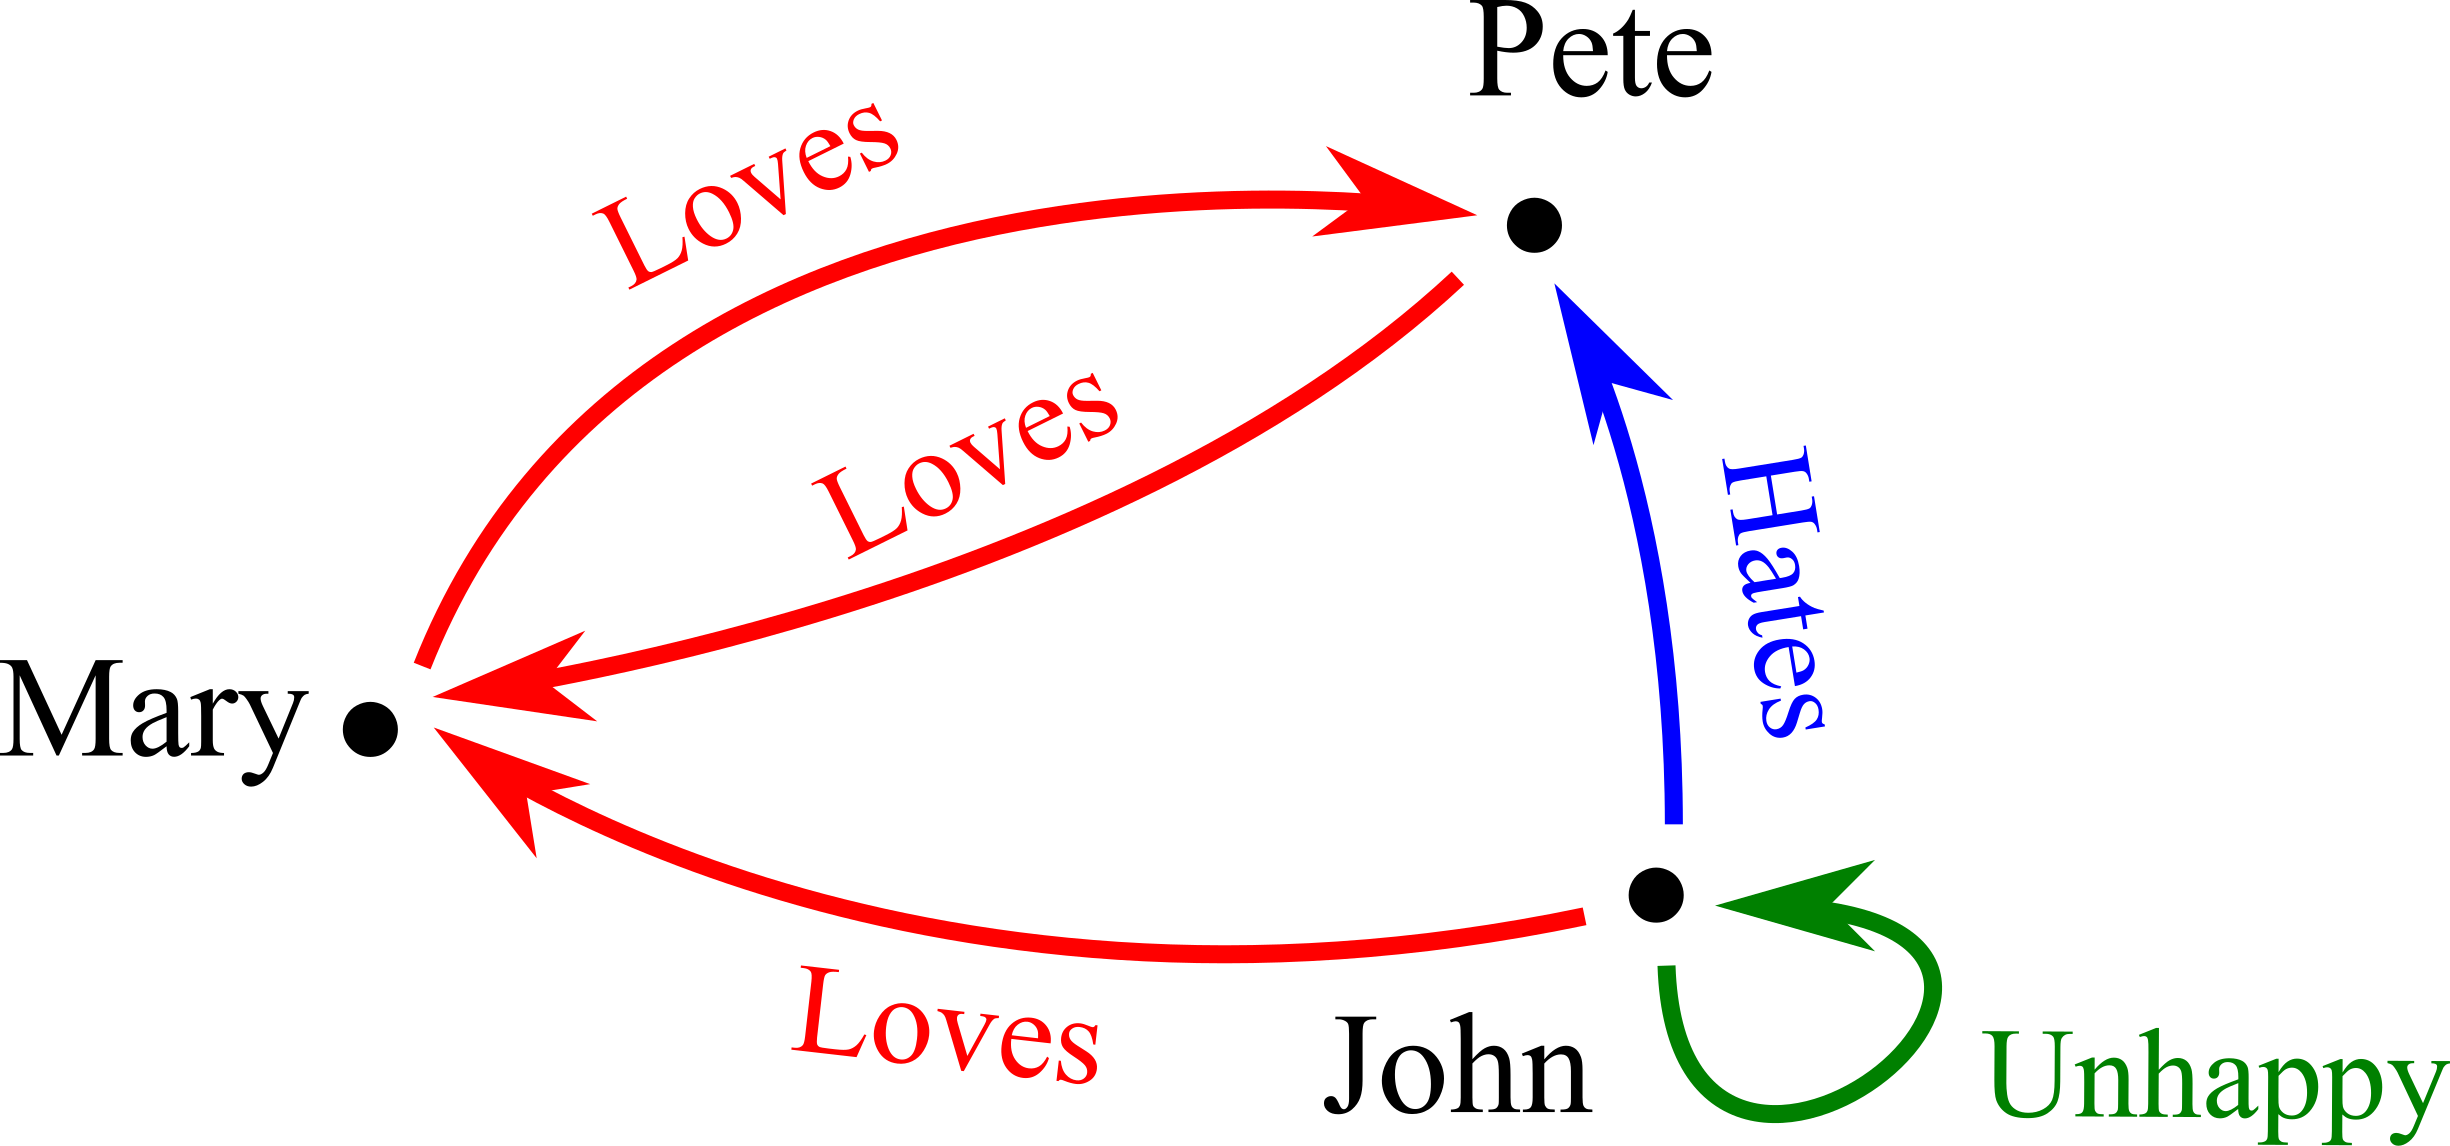
\includegraphics[scale=0.5]{FOL-model-3.png}}} 
\end{equation}
This is a \textbf{directed multi-graph}, or \textbf{quiver}. Quiver is an important structure in algebraic representation theory. The category of quivers $\mathcal{Q}$ is a \textbf{topos} (this is introduced in the
% \S\ref{Categorical-semantics}), 
the basic meaning is \uline{it has conditional first-order logic as }\textbf{\uline{model}}\uline{ category} \footnote{According to \parencite{Grilliette2017}, hyper-graph is not topos, multi-graph is not topos, but when they become directed. } .

The above knowledge graph can be simply converted to a collection of \textbf{logical children}:
\footnotesize
\begin{equation}
\begin{array}{l}
	\verb|Loves(John, Mary)| \\
	\verb|Loves(Pete, Mary)| \\
	\verb|Loves(Mary, Pete)| \\
	\verb|Hates(John, Pete)| \\
	\verb|Unhappy(John)|
\end{array}
\label{FOL-model}
\end{equation}
\normalsize
So, \uline{logic and graph are basically }\textbf{\uline{equivalent}}.
\begin{tcolorbox}[breakable, parbox=false]
If each edge of graph can contain any number of vertices, then there is \textbf{hyper-graph}. In other words, each edge of the hypergraph $\in \powerset(V)$, $V$ is the vertex set. It can also be said that the hypergraph is the \textbf{ subset system} of V. For logic, the benefit is: \uline{There can be relationships on the relationship}.
Hypergraph can correspond to the topological \textbf{simplicial complex}, and its homology and cohomology can be studied. The Simplicial complex can also correspond to \textbf{square-free monomial ideals} one-to-one. Square-free means that the index of $x_i$ can only be 0 or 1. The latter is the scope of the \textbf{combina commutative algebra}. For the time being, I don't know if these associations are useful. See \parencite{Brown2013}, \parencite{Miller2005} for details.\end{tcolorbox}

A collection of logical expressions is called logical \textbf{theory}. A collection of algebraic equations is called \textbf{algebraic theory}.
For example, you can have the following logical formula (``love is not happy''):\begin{equation}
\forall x,y. \; \mbox{Loves}(x,y) \wedge \neg \mbox{Loves}(y,x) \rightarrow \mbox{Unhappy}(x)
\end{equation}
This formula contains universal quantification, so it is not part of the model. Logically, only the collection of \textbf{ground sentences} (the expression without variables) can form a model, for example (\ref{FOL-model}) .

\section{Fractal structure of model space}

An expression in Logic \textbf{theory} can cause many \textbf{new} vertices and joins to appear in the model. This is a question of model theory research. In some cases, the model space will have an "infinitely subdivided" fractal structure.
For example, each natural number $n \in \mathbb{N}$ has its successor $S(n)$. The existence of this function causes a series of \textbf{infinite} vertices in the model space:
\begin{equation}
\textbullet \quad \textbullet \quad \textbullet \quad \textbullet \quad \textbullet \quad \textbullet \quad \textbullet \quad \textbullet \quad \textbullet \; .....
\end{equation}
If you add this \textbf{rule}:\begin{equation}
\forall n \in \mathbb{N}. \quad S(n) \ge n
\end{equation}
Then immediately generate an infinite number of relationships:
\begin{equation}
\textbullet \stackrel{\ge}{\longleftarrow} \textbullet \stackrel{\ge}{\longleftarrow} \textbullet \stackrel{\ge}{\longleftarrow} \textbullet \stackrel{\ge}{\longleftarrow} \textbullet \stackrel{\ge}{\longleftarrow} \textbullet \stackrel{\ge}{\longleftarrow} \textbullet \stackrel{\ge}{\longleftarrow} \textbullet \; .....
\end{equation}
Although, in \textbf{common-sense intelligence}, it seems that this infinite structure is less common, and more is the structure of ``shallow''.
\footnotesize
Incidentally, the knowledge representation of classical logic-based AI is split into two parts: \textbf{rules} and \textbf{facts}. The former is the formula with $\forall$ \textbf{variable}, the latter is ground sentences. Rules are stored in $\KB$ and facts are stored in \textbf{working memory}. The former is a \textbf{theory}, which can be thought of as some \textbf{``partial'' models}. The reason for saying partial is because it does not represent the entire model. In fact, model is a very large thing that cannot be stored in a physical system. Artificial intelligence or the brain can only store certain theories and parts of models. The key issue of artificial intelligence is how to find a good syntax structure to make theory learning faster and more efficient.\normalsize

\section{A concise formulation of strong AI}

This section describes the mathematical structure of a strong artificial intelligence system in a way that is as concise as possible, even if the mathematician without an AI background can understand it.
\begin{tcolorbox}[breakable, parbox=false]
Revisit \textbf{neural network} like this:\begin{eqnarray}
\mbox{\footnotesize 每层的} \tikzmark{ww} \mbox{\footnotesize \textbf{权重}矩阵} \quad \quad \mbox{\footnotesize 总层数} \tikzmark{LL} \nonumber \\
\nonumber \\
F(\vec{x}) = \sigmoid(W_1 \tikzmark{wa} \sigmoid(W_2 \tikzmark{wb} ... \sigmoid( W_L \tikzmark{wc} \tikzmark{L} \; \vec{x} )))
\begin{tikzpicture}[overlay,remember picture]
  \draw[-, shorten <=12pt, transform canvas={shift={(-10pt,10pt)}}] (ww.center) to (wa.center);
  \draw[-, shorten <=16pt, transform canvas={shift={(-10pt,10pt)}}] (ww.center) to (wb.center);
  \draw[-, shorten <=28pt, transform canvas={shift={(-10pt,10pt)}}] (ww.center) to (wc.center);
  \draw (LL.center) +(-15pt,-3pt) -- ([shift={(-2pt,6pt)}]L.center);
\end{tikzpicture}
\end{eqnarray}
Its \textbf{parameter} collection $\Theta = \{ W_{i, j}^{\ell} \} \in \mathbb{R}^m$, where $m$ = \# weights.
The purpose of \textbf{machine learning} is to \uline{find optimal $\Theta$ subject to an objective function}. In other words, machine learning = \textbf{optimization}, which is one of the most basic problems in applied mathematics.
When training, give a set of data points ($F$ is a neural network):\begin{equation}
\label{NN-training}
\boxed{\mbox{training examples}} \quad
e \stackrel{F}{\longrightarrow} a
\quad \boxed{\mbox{answers}} 
\end{equation}
The error for each answer is $\epsilon$, and the objective function $J$ is the sum of the errors of many iterations.% \begin{equation}
% J = \sum_t \epsilon \; ( e, a, \Theta )
% \end{equation}
We want to optimize $J$ by calculating the gradient of $J$ for $\Theta$:\begin{equation}
\nabla_{\Theta} J := \frac{\partial J}{\partial \Theta}
\end{equation}
当然这就是著名的 back-propagation 算法,其实即 gradient descent。
\end{tcolorbox}

\begin{tcolorbox}[ams equation, colback=yellow, colframe=white]
\mbox{强人工智能 的樽颈问题 是\textbf{学习算法}的速度}
\end{tcolorbox}

The feature of the AI learning algorithm is that \uline{ needs to be optimized on }\textbf{\uline{ logical sub}}:
\begin{tcolorbox}[ams align, colback=yellow, colframe=white]
\mbox{从 } \mbox{ optimization over $\mathbb{R}$} && \mbox{ 过渡到 } & \mbox{ optimization over $\mathcal{L}$} \nonumber\\
\Theta \in \mathbb{R}^m && \rightsquigarrow & \; \; \Theta \in \mathcal{L}
\end{tcolorbox}
Where $\mathcal{L}$ is some sort of (eg first-order predicate) \textbf{logical syntax}, and $\Theta$ is a collection of logical children. The solution to this optimization problem $\Theta^*$ is an optimal logic theory.
The top-level architecture of the system is reinforcement learning, which is dynamic programming. It is a special case of optimization. It can also be called control theory. The \textbf{system} it controls is:\begin{equation}
\vec{x}_{n+1} = \vec{f}( \vec{x}_n, \vec{u}_n )
\end{equation}
$\vec{x}$ is the system's \textbf{status}, and $\vec{u}$ is called control or action. In AI, $\vec{x}$ is the \textbf{location} in the "think space", and $\vec{u}$ is the "thinking" step. We want to control $\vec{u}$ so that the system reaches the maximum value of \textbf{rewards} in \uline{long running}:\begin{equation}
\boxed{\mbox{total rewards}} \quad J = \sum_n L(\vec{x}) = \int L dt
\end{equation}
$L \in \mathbb{R}$ is the \textbf{instant reward} at the $\vec{x}$ position. Based on historical analysis mechanics, $L$ is also called \textbf{Lagrangian}, unit It's energy (but the sign changes, the latter measures the penalty), but note that $\vec{x}$ is a "think space", unlike physical space. I am writing a differential form to make it easier to remember.
The system operates as follows:\begin{equation}
\vcenter{\hbox{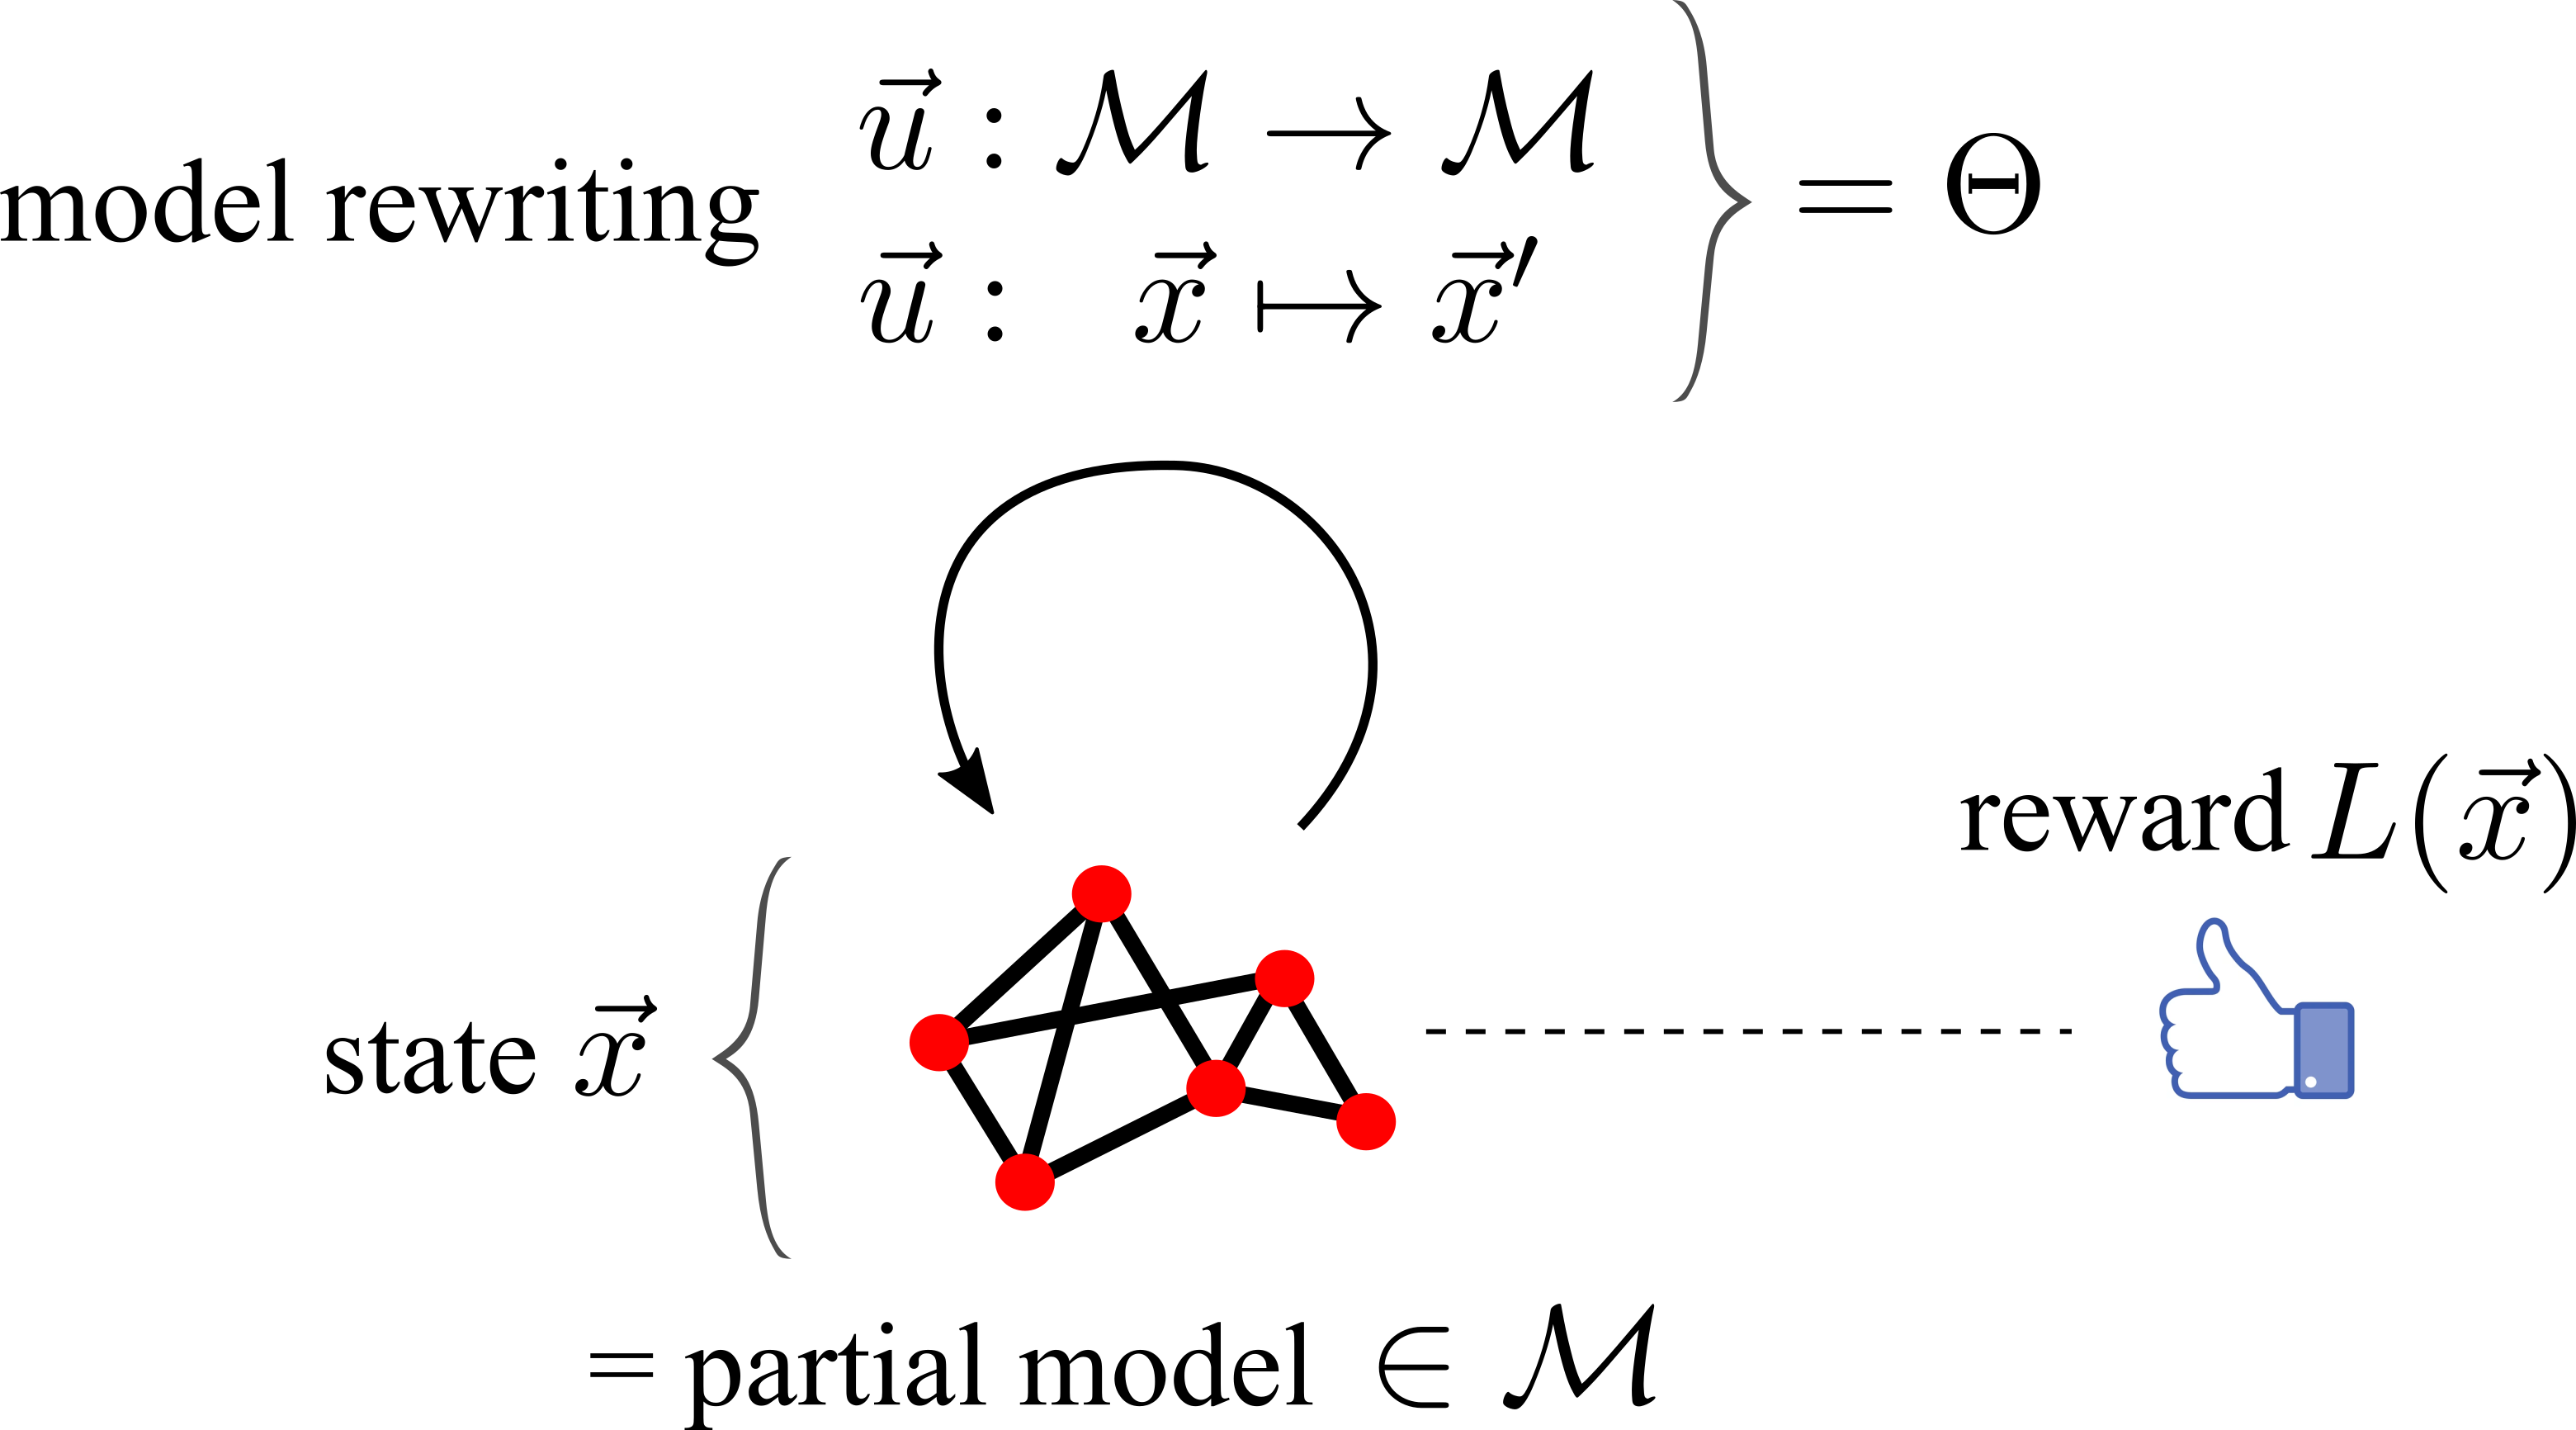
\includegraphics[scale=0.7]{abstract-dynamic-programming.png}}}
\end{equation}
% $\vec{x}$ 的某些部分用作\textbf{输出},经由它得到奖励。 
$\vec{u}$ and $\vec{f}$ coincide, the function is to \textbf{rewrite} $\vec{x}$:
\begin{equation}
\vec{f}(\vec{x},\vec{u}) \equiv \vec{u}(\vec{x})
\end{equation}
For example, the logic rule ```失恋 $\Rightarrow$ 不开心'' performs the rewriting of the following sub-graph:\begin{equation}
\vcenter{\hbox{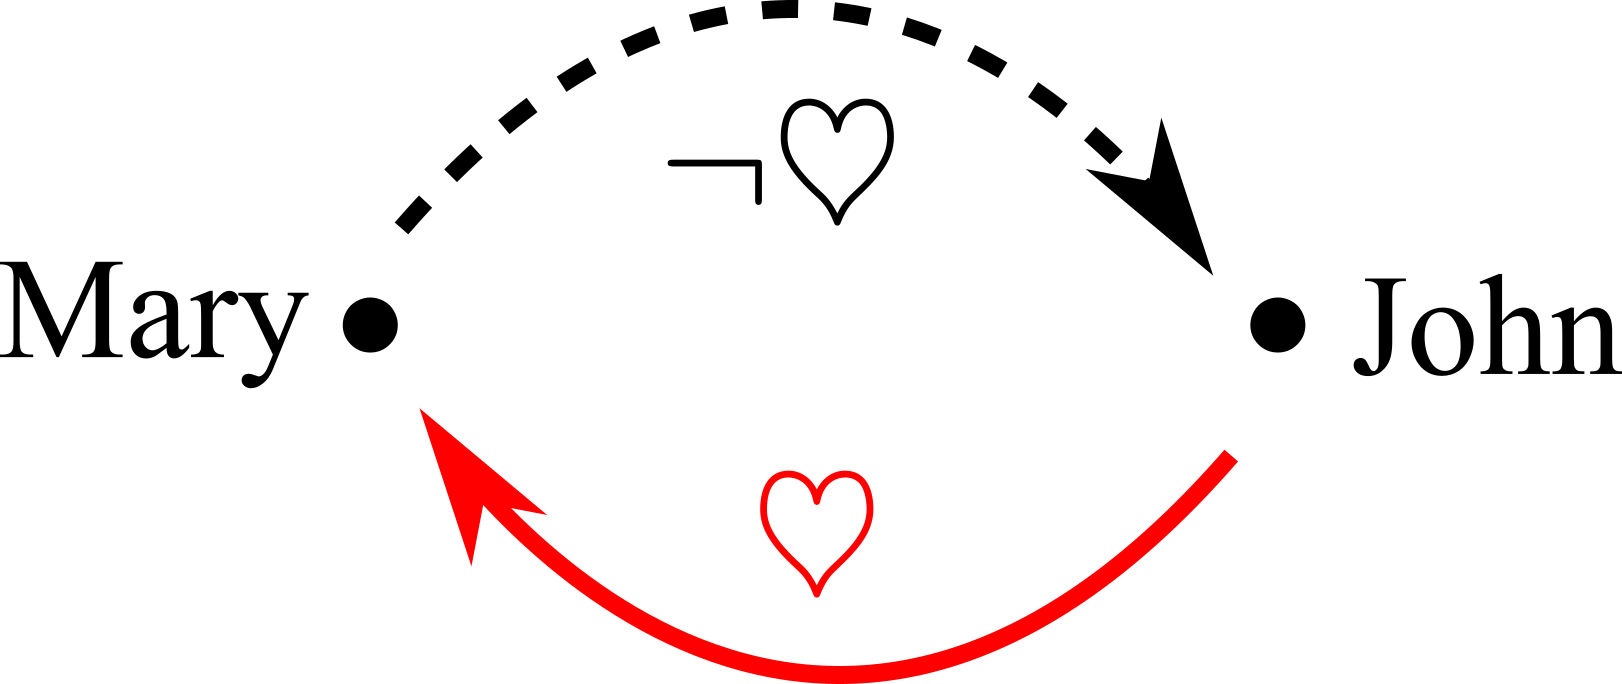
\includegraphics[scale=0.6]{heartbreak-precond.png}}}
\quad \mapsto \quad
\vcenter{\hbox{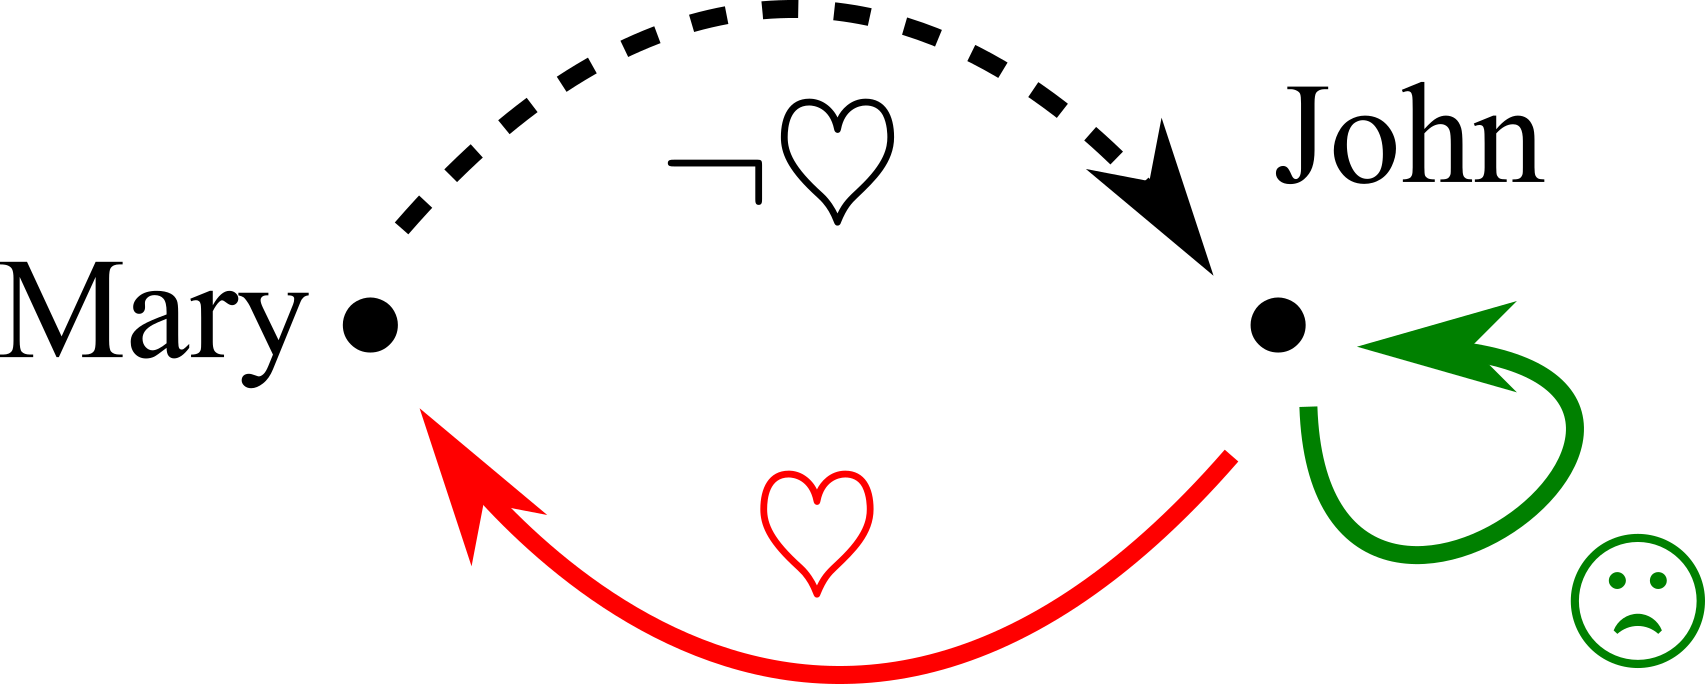
\includegraphics[scale=0.6]{heartbreak-postcond.png}}}
\end{equation}
This is the \textbf{state transition} $\vec{u}: \vec{x} \mapsto \vec{x}'$, which can also be regarded as the \textbf{logical inference} $\vec{u}: \vec{v} \vdash \vec{x}'$, where $\vec{u}$ is the rewriting function or logic rule.
Optimization of $J$ acts on top of $\Theta$ (ie $\vec{u}$). Note that $\vec{u} \in$ is a function space or logical formula, which is very different from the traditional optimization over $\mathbb{R}$.
\footnotesize
In classic AI, $\vec{u}(\vec{x}) = \vec{f}(\vec{x})$ is equivalent to deduction $\vec{x} \vdash \vec{x} '$, or forward-chaining (forward some logical conclusions). In classic AI this work is handled by \textbf{logic engine}, which contains two algorithms: \textbf{unification} (= rule matching) and \textbf{resolution} (= proof search). These operations are not visible in our framework because they are included in $\vec{u}$ or $\vec{f}$.\normalsize

%训练的过程类似 (\ref{NN-training}):
%\begin{equation}
%\boxed{\mbox{training examples}} \quad
%e \sststile{}{\Theta} a
%\quad \boxed{\mbox{answers}} 
%\end{equation}
%但现在 $\vdash$ 是根据 $\Theta$ 的 \textbf{逻辑推导},$e$ 和 $a$ 是逻辑式子的集合。 给定一些前提,可以推出很多结论,其中有些得到奖励或惩罚。 % 在 \textbf{强化学习} (reinforcement learning,亦即 dynamtic programming) 的框架下,训练是根据 \textbf{奖励} 而不是 \textbf{误差},和上面略有不同。 

For experts in applied mathematics, the following theory is quite standard. The definition of Hamiltonian in analytical mechanics is:\begin{equation}
H = L + \frac{\partial J}{\partial \vec{x}} \vec{f}
\end{equation}
Similarly, the Hamiltonian of the \textbf{discrete} system can be defined as:\begin{equation}
H = L + J ( \vec{f}(\vec{x}) )
\end{equation}
Pontryagin\footnote{Lev Pontryagin (1908-1988) Soviet mathematician. Blind since the age of 14, he made major discoveries in a number of fields including algebraic topology and differential topology.} 的 \textbf{极小值原理} 给出最优解的条件是:\begin{equation}
\label{Pontryagin-max-principle}
H^* = \inf_u H \quad \mbox{or} \quad \nabla_{\vec{u}} H^* := \frac{\partial H^*}{\partial \vec{u}} = 0
\end{equation}
可以定义一个作用在 J 上的算子 T:
\begin{equation}
T J := \inf_u H
\end{equation}
Then Bellman's optimality condition can be expressed as the following fixed-point form \parencite{Bertsekas2013}:
\begin{equation}
J^* = T J^*
\end{equation}
It is said that the Hamilton-Jacobi method leads to the solution of partial differential equations, which is not particularly effective. In practice, the Pontryagin minimum principle is more useful.
There is a gradient $\nabla_{\vec{u}}$ in (\ref{Pontryagin-max-principle}), so it would be useful to find a derivative for $\vec{u}$. If the problem is continuous optimization, you can use non-smooth analysis. The minimum requirement is that there is norm (\textit{ie}, Hilbert space or Banach space) on the domain, you can use the method such as proximal gradient.
The key issue is: $\Theta$ belongs to a domain other than the traditional $\mathbb{R}^n$.

\section{Plan 0: geometric models}

\begin{tcolorbox}[ams equation, colback=yellow, colframe=white]
\mbox{一阶逻辑语法 $\mathcal{L}$ 不是必需的,只需某种将 model \textbf{改写} 的能力}
%\uline{一阶逻辑语法 $\mathcal{L}$ 不是必需的,只需要某种将 model }\textbf{\uline{改写}}\uline{的能力}。 
\end{tcolorbox}
There can be many different variants, for example:\begin{equation}
\begin{tikzcd}[column sep = large]
\mbox{逻辑语法 } \; \mathcal{L} \arrow[d] \\
\mbox{partial model } \mathcal{M}
\end{tikzcd}
\approx
\begin{tikzcd}[column sep = large]
\mbox{graph re-writer} \arrow[d] \\
\mbox{graph model}
\end{tikzcd}
\end{equation}

Consider a model I call \textbf{geometric model}, for example:
\begin{equation}
P(x) \wedge Q(x) \quad \cong \quad
\vcenter{\hbox{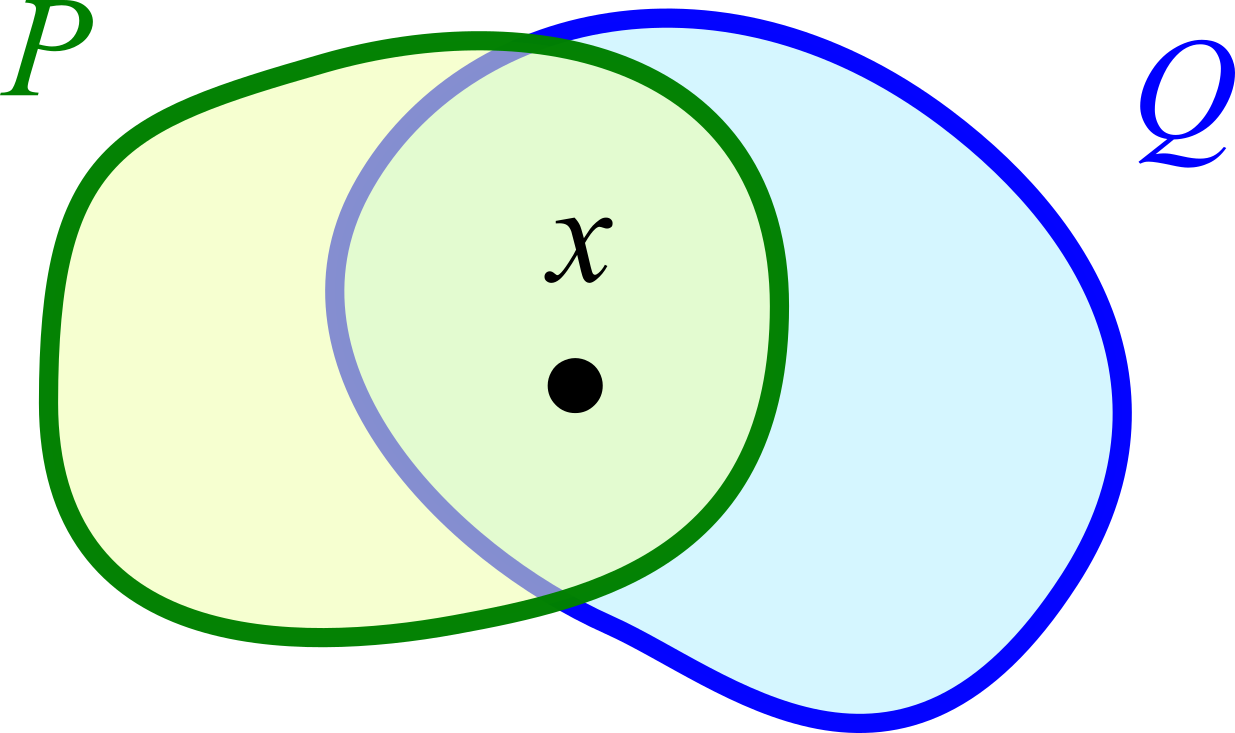
\includegraphics[scale=0.7]{Venn-diagram.png}}}
\end{equation}

These geometric ``\textbf{regions}'' are easy to do with neural networks. If $\vec{F} =$ neural network, then:
\begin{equation}
\vec{F}(\vec{x}) = 0
\end{equation}
定义了一个 hyper-surface of co-dimension 1,它将周围的空间分割为 $> 0$ 和 $< 0$ 两部份。 

One effect that you hope to achieve (but perhaps hard to do) is: \uline{a logical formula can be deformed into another different expression}. This is not possible in classic logic, such as $\mbox{Love}(x,y)$ and $\mbox{Like}(x,y)$, although the meaning is close, but from one to the other must be discrete Jumping. As shown below, two approximate regions:
\begin{equation}
\vcenter{\hbox{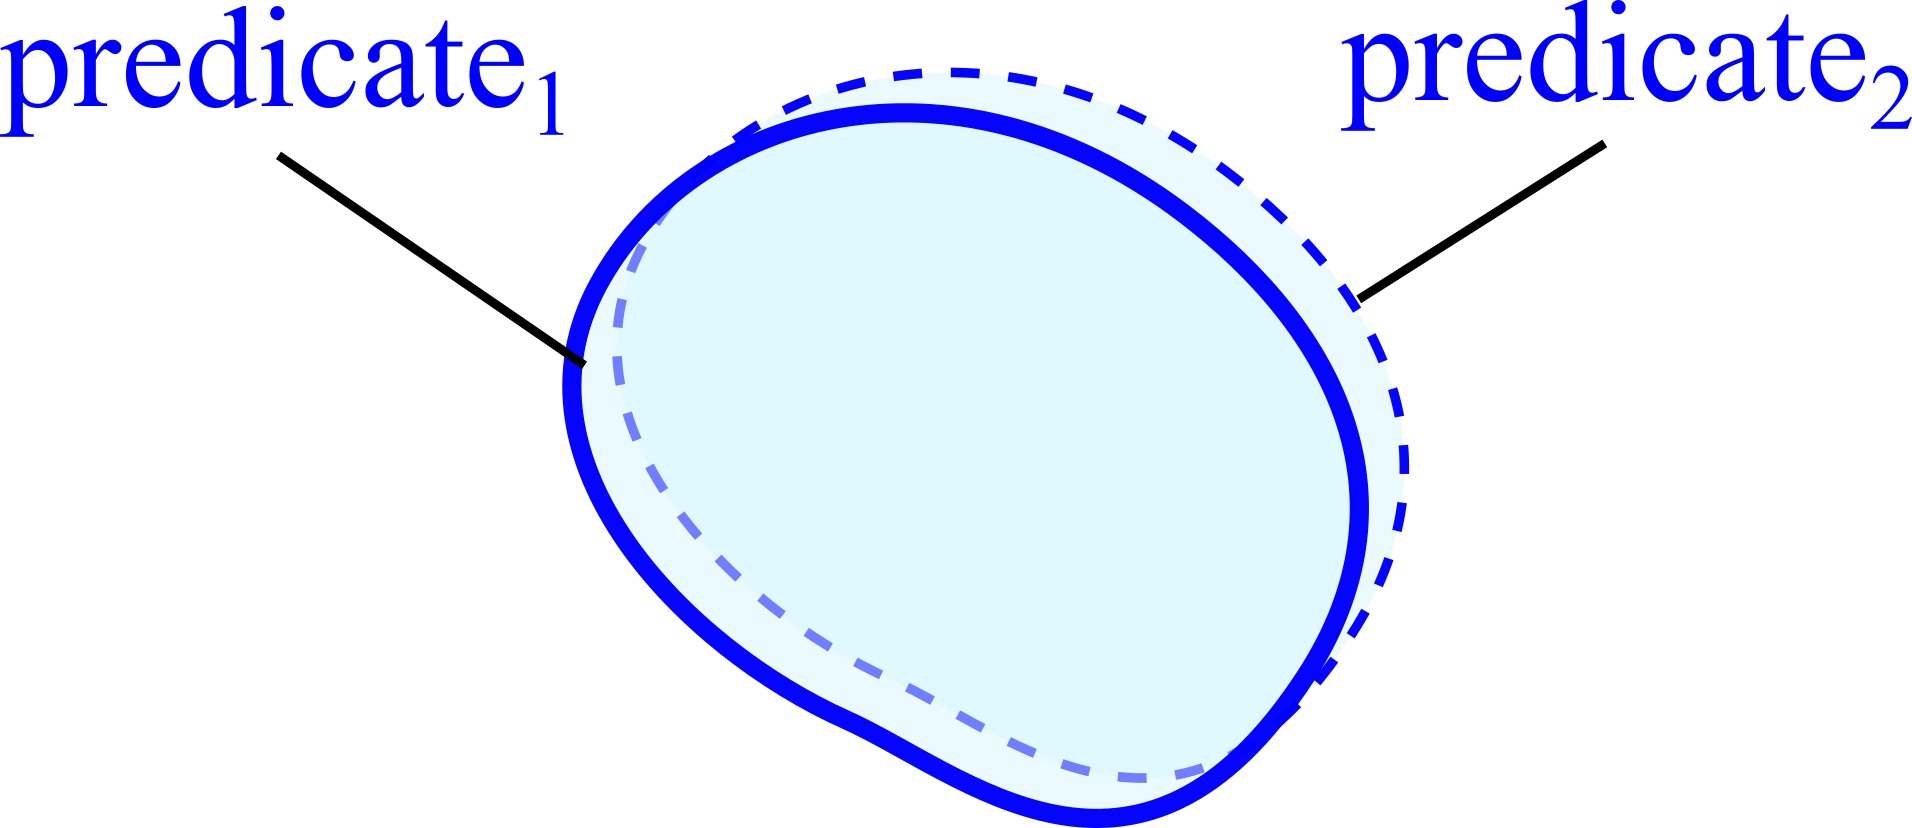
\includegraphics[scale=0.7]{nearby-predicates.png}}}
\end{equation}
它们是不是两个 distinct objects 视乎 representation 怎样而决定。

% 根据 范畴论 的看法,一个集合里的\textbf{元素},是一个 $\mathbf{1} \rightarrow \mathbf{Set}$ 的 mapping。  如果我们不想要「一粒粒」的元素,或许可以用 $\mathbb{R} \rightarrow \mathbf{Set}$ 这样的 mapping? 

In summary, this program is:
\begin{eqnarray}
\mbox{model } \mathcal{M} &=& \mbox{geometric model of set theory} \nonumber \\
\mbox{rewriter} &=& \mbox{functor } \mathcal{M} \rightarrow \mathcal{M}
\end{eqnarray}
But we need a \uline{model of set theory that can be continuously changed}, maybe it can be achieved with some kind of fuzzy topology? E.g:
\begin{equation}
\vcenter{\hbox{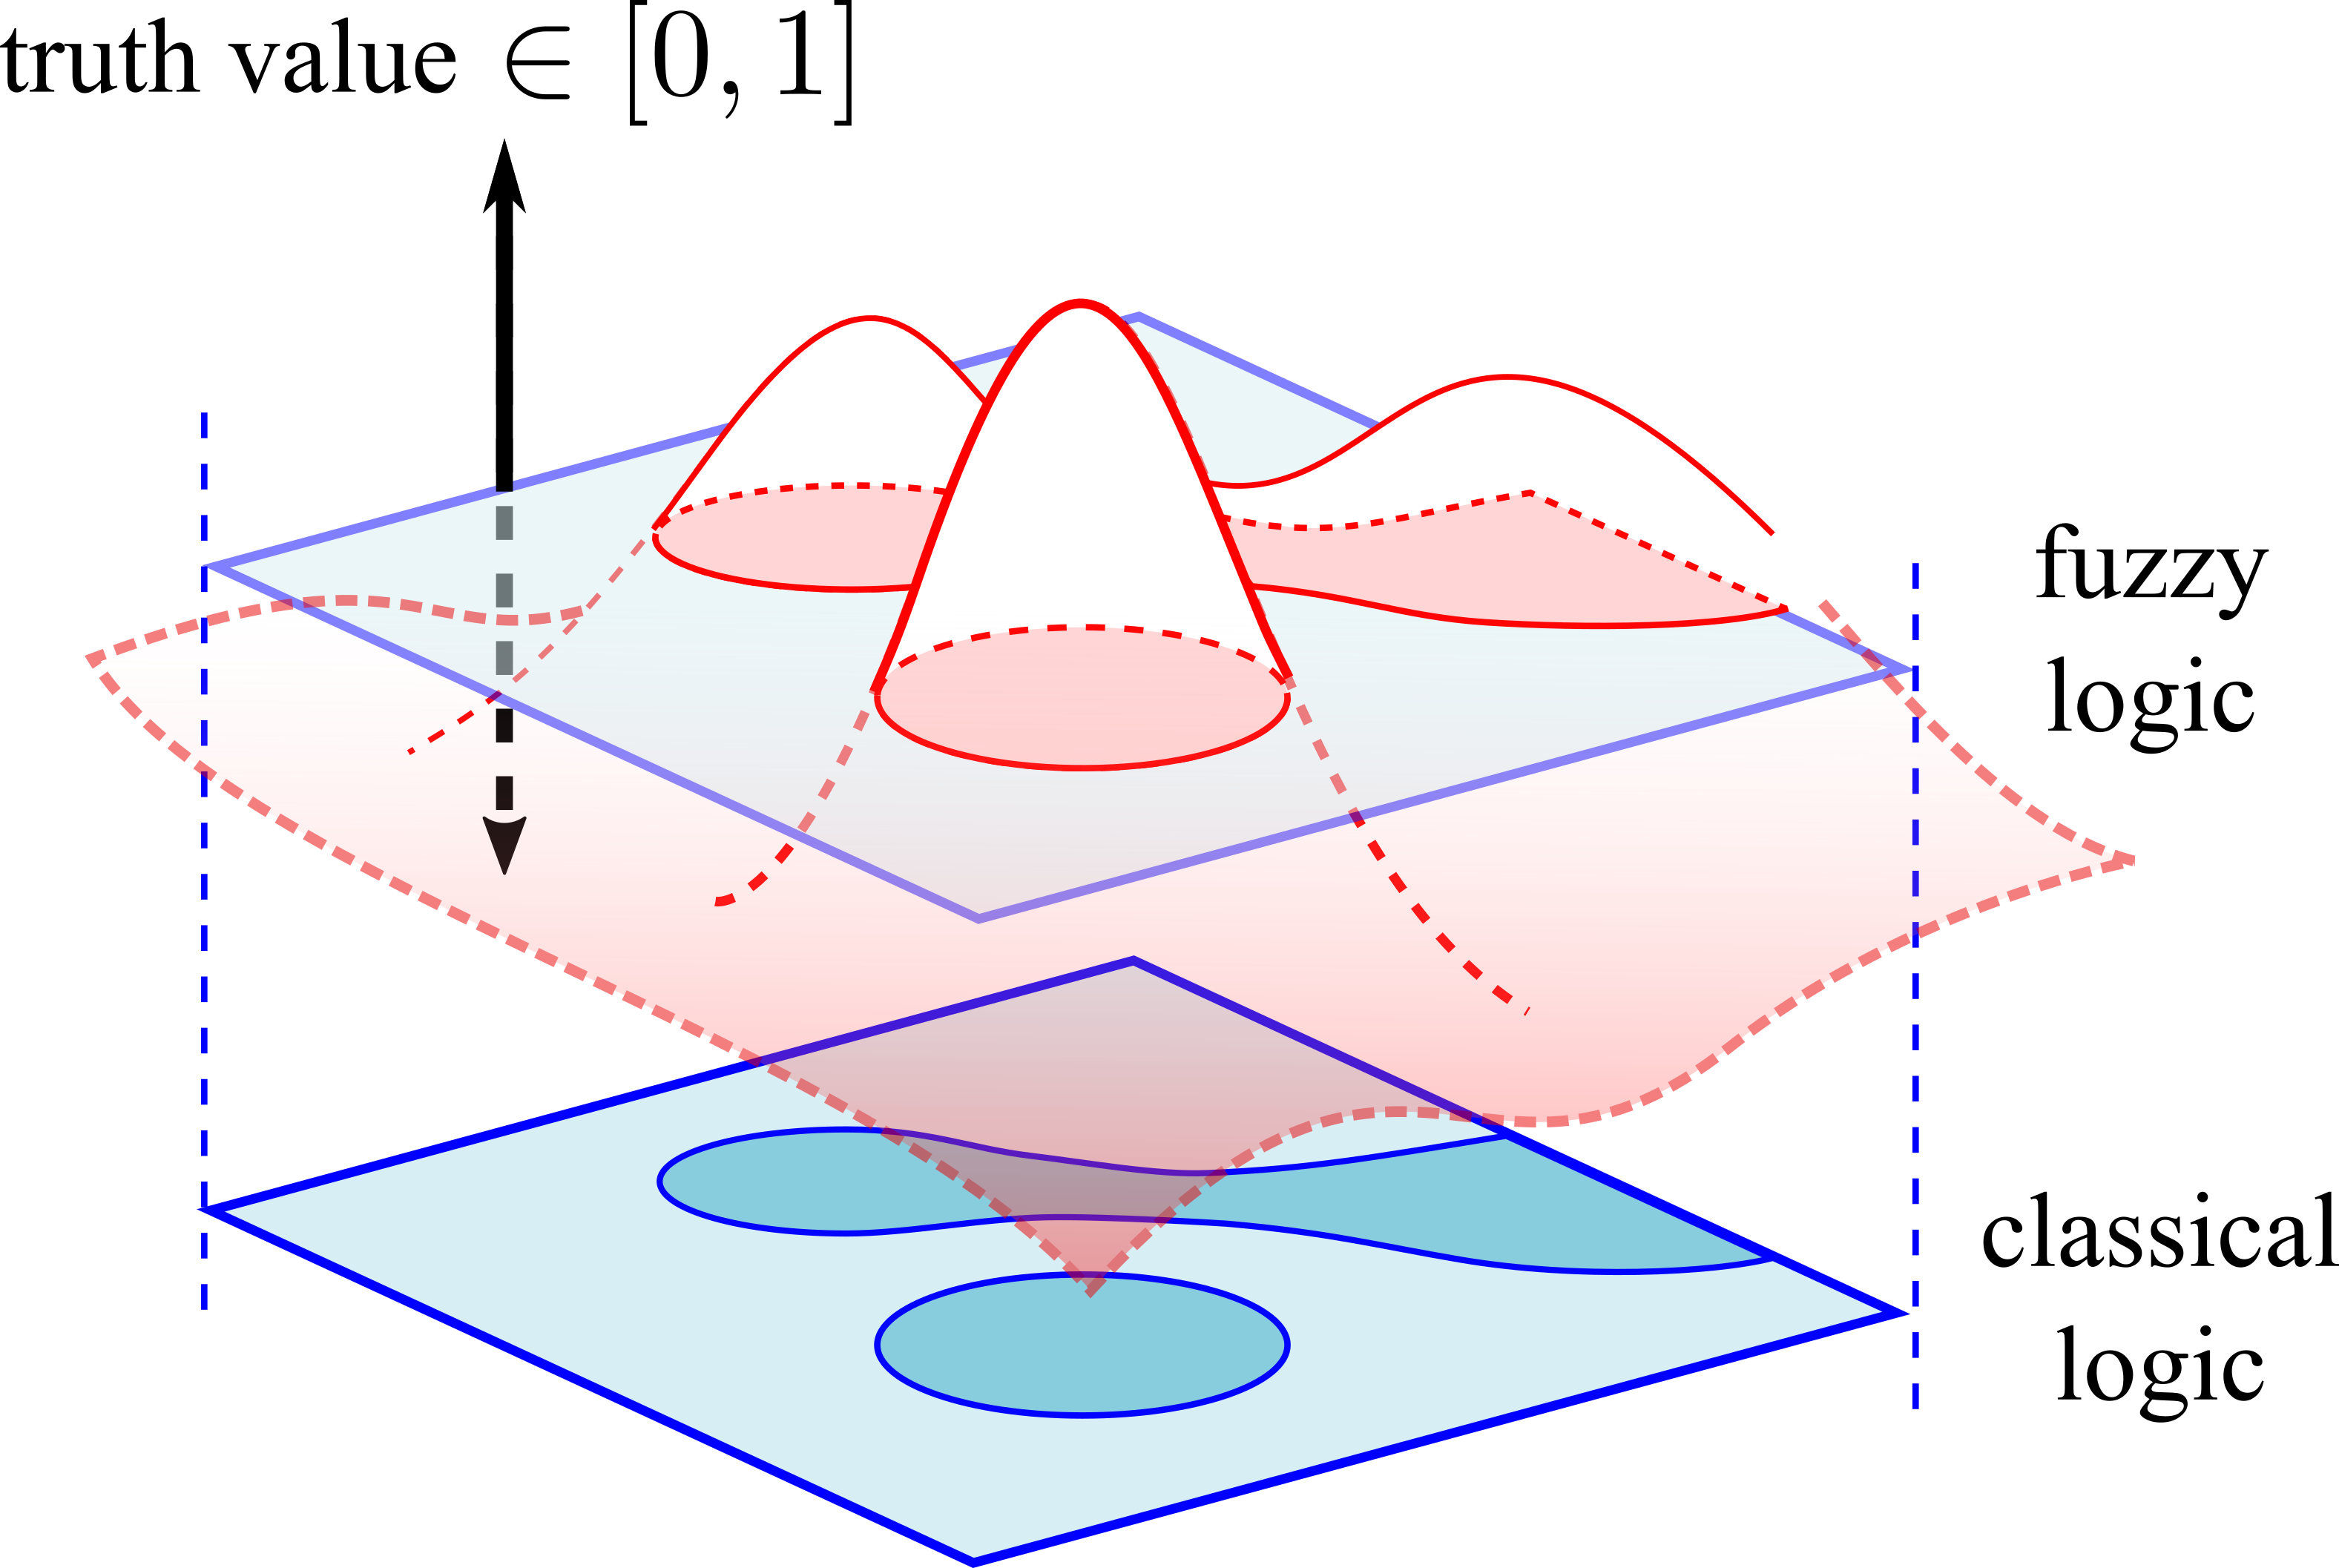
\includegraphics[scale=0.7]{fuzzy-geometric-model.png}}}
\end{equation}
% 和传统 fuzzy logic 不同,我将 ``neutrality'' $\frac{1}{2}$ 移到 0 的位置,这样更符合直观。 
The boundary of regions that need to be defined is 1 degree higher.

\footnotesize
But here's the problem: Logically, the semantic distance between two expressions can be defined as the number of proof steps required to derive from one formula to another (it also depends on the other within $\KB$ (), but according to the halting problem theorem that Turing proved in 1936, this distance is \textbf{uncalculable}. \footnote{The logic semantic distance is similar to \textbf{Kolmogorov complexity} but not exactly the same. Kolmogorov complexity is incomputable but can be approximated \parencite{Li2008}.} In other words, it is impossible in the space of the logical subroutine There is a fully defined semantic metric. Our $\vec{u} = \Theta$ is similar to a logical subroutine. If we can define gradient $\nabla_\Theta$ on $\Theta$, it seems to be contradictory. Will \textbf{fuzzy topology} be able to approximate the semantic metric? This depends on the fuzzy writing model's rewriting function space $\Theta$ is not \textbf{metrizable} (\textit{cf} \parencite{Goubault-Larrecq2013}). I will study this in more detail in the future.
\normalsize
\begin{equation}
\vcenter{\hbox{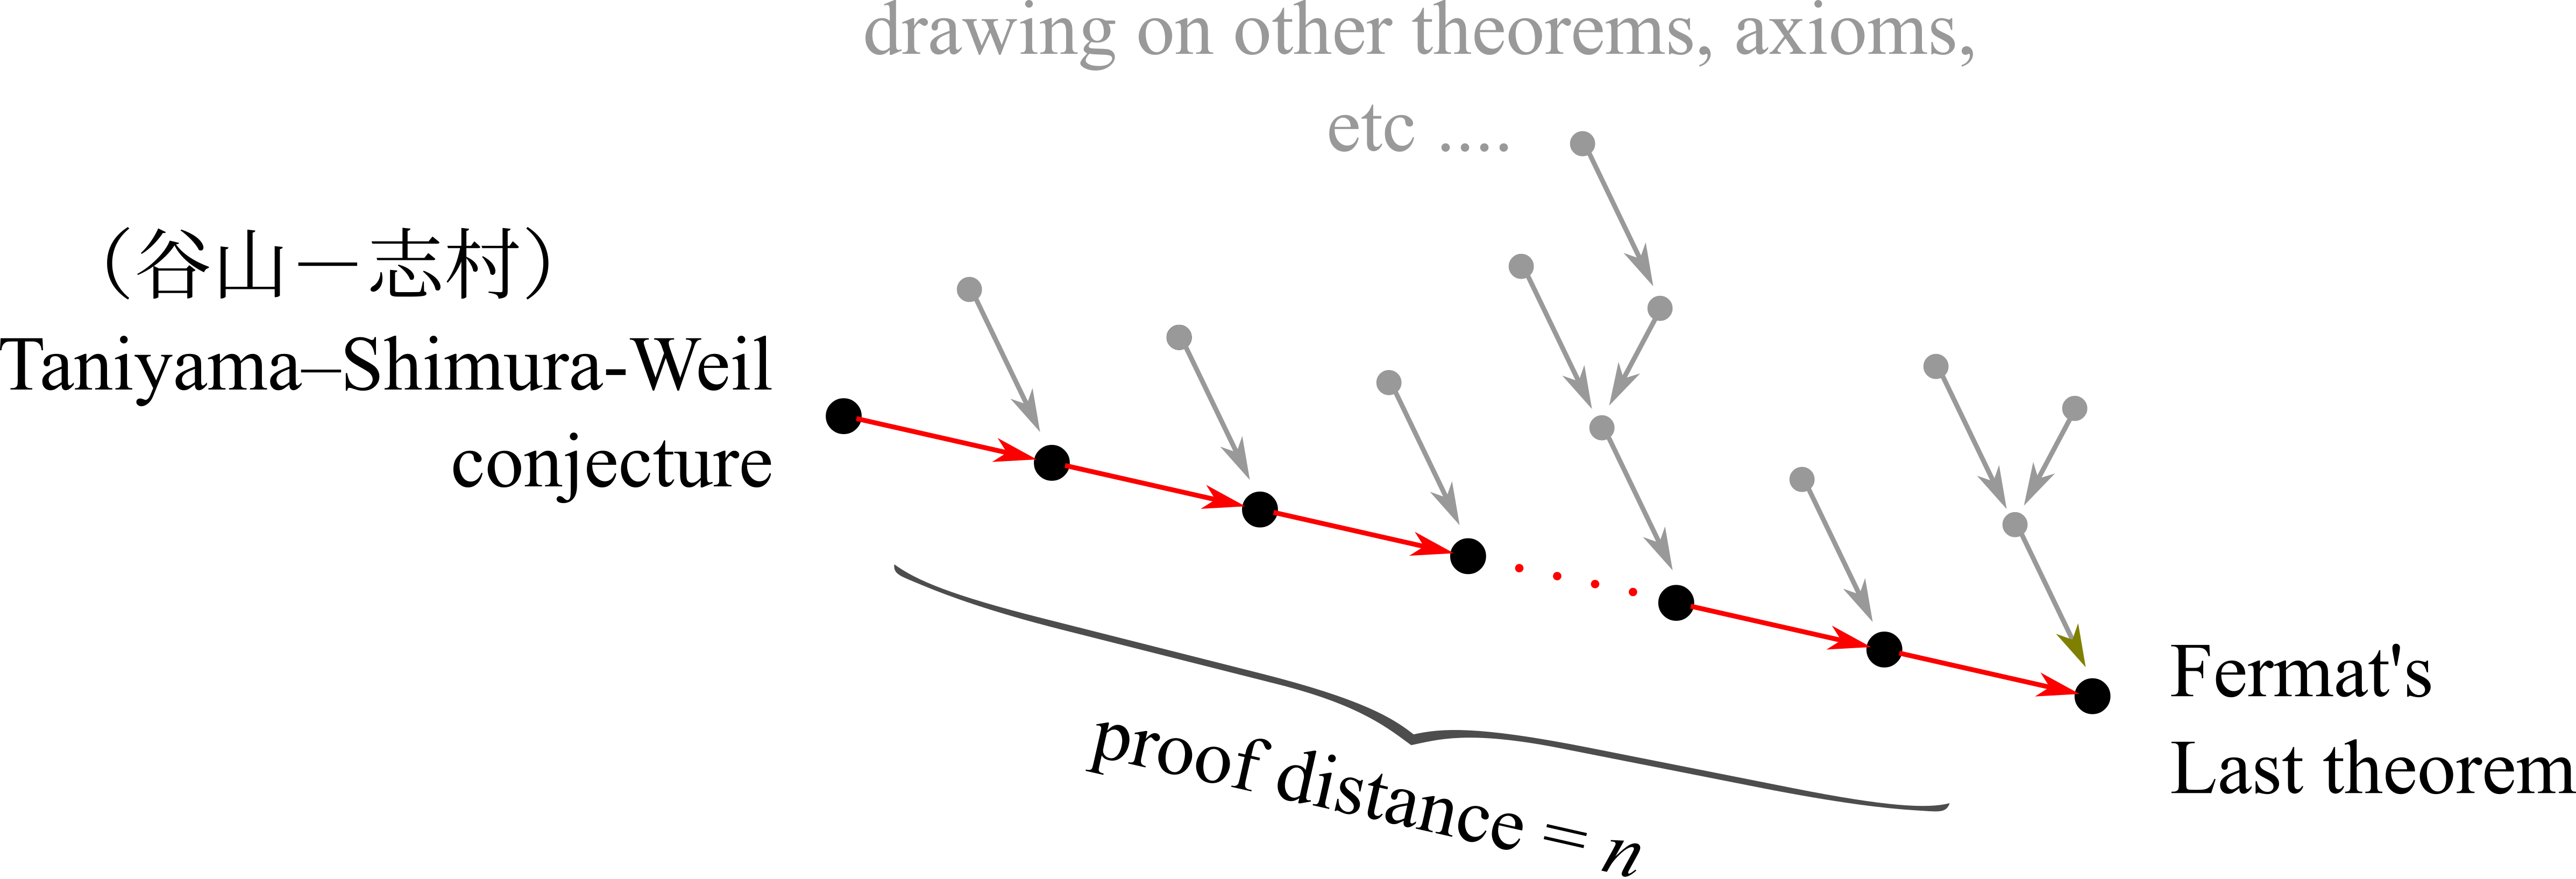
\includegraphics[scale=0.6]{proof-distance.png}}}
\end{equation}

% 如果想用传统的 基於 differentials 的 optimization 技巧,似乎最低要求是 domain 上的 topology、continuity 和 compactness,然后才可以定义例如 Fr\'{e}chet derivative. \parencite{Henrot2018}

% 当然,如果改写的能力太弱,则会 ``throw the baby out with the water'',亦即丧失了一阶逻辑的\textbf{泛化}能力。  同时,要从 optimization 的角度考虑,什么形式的改写才最有利於速度。  模型的 representation 也是一个考虑因素: 它应该有某种良好的 \textbf{metric},这 metric 近似 semantic distance,而不是纯粹基於 logic syntax。 事实上,完美的 semantic metric 是\textbf{不可计算的},因它是 Kolmogorov complexity.

\begin{center}
\rule{0.4\textwidth}{.6pt}
\end{center}

The following main analysis of plan A and B (they are already feasible). Plan A uses discrete optimization directly, so no metric space is required. Plan B uses a neural network whose weights $\in \mathbb{R}$ is a contiguous space, but this neural network acts on the graph, which is still a discrete structure.

\section{Plan A: genetic algorithm}
\label{COCO}

\begin{tcolorbox}[ams equation, colback=yellow, colframe=white]
\mbox{放弃梯度下降}
\end{tcolorbox}
\begin{eqnarray}
\mbox{model } \mathcal{M} &=& \mbox{符号逻辑式子} \nonumber \\
\mbox{rewriter} &=& \mbox{符号逻辑式子 + 经典 AI 逻辑引擎}
\end{eqnarray}

GA is very suitable for the \textbf{discrete} search space. It is compatible with the logical structure. There is no theoretical obstructions on this route.
% \section{Plan A: 协同进化 (COCO)}

% Substitution 的麻烦令我想到 \uline{放弃用 neural network 直接处理逻辑,而是用 hybrid 的 神经/逻辑 混合}: 视觉神经用 deep neural network,到高层次转用符号逻辑表述,后者用 genetic algorithm 做学习。

First you need a logic-based \textbf{rule engine}, which is responsible for forward-chaining, which is completely the scope of classic AI. For example, the classic Soar architecture [Carnegie-Mellon University] is a rule-base engine. % and my generation of OpenCog, OpenNARS, and my Genifer\footnote{Genifer have not yet reached the production stage.}, and perhaps a newer generation of AGI systems (?)
% 经典逻辑 AI 的樽颈问题是 \uline{rules 的学习算法太慢},
%\begin{itemize}
%\item plan A: 继续用经典逻辑引擎,用 genetic algorithm 做学习算法
%\item plan B: 将逻辑记忆映射到向量空间,再用神经网络学习逻辑 rules
%\end{itemize}

The genetic algorithm's population is composed of individual logical rules, but the winner is not a single rule, but a set of rules (the highest score of $N$). This is called \textbf{cooperative co-evolution}(COCO).
Inputs and outputs are logic formulas, which are actually easier to handle.
The whole system is still based on reinforcement learning, but you don't need to do RL directly, because those rules are actually \textbf{actions}, and the probabilistic strength of each rule is like the $Q$ value in $Q$-learning.
[I have not had time to explore the practical theory of COCO. ]

\section{Plan B: neural network / deep learning}

Most of the time is to solve the problem of how to implement the classic logic engine with NN, especially the problem of variable substitution. Finally, the crux of the problem is the lack of short-term memory mechanism.
The solution is to use graph as \textbf{memory system} and use neural network for graph re-writing, which is the graph neural network proposed by Google / DeepMind. This is a ``hybrid'' architecture.

\subsection{Neural networks has difficulty handling substitutions}
\label{NN}

Consider the logic rule that was mentioned in the previous section (``Love is not happy''):\begin{equation}
\forall x,y. \; x \heartsuit y \wedge \neg y \heartsuit x \rightarrow \frownie{} x
\end{equation}
The \textbf{predecessor} (antecedent) of this rule must be established, and must be \uline{$a$ }\textbf{\uline{equal}}\uline{, twice appearing, $b$ }\textbf {\uline{equal}}:\begin{equation}
\vcenter{\hbox{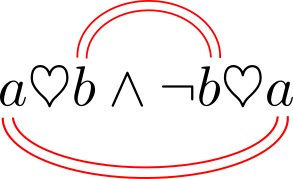
\includegraphics[scale=0.6]{antecedents-equal.png}}}
\end{equation}
Also, to produce the correct \textbf{postsent} (consequent), you need to pass $a$ \textbf{copy} from the previous:\begin{equation}
\vcenter{\hbox{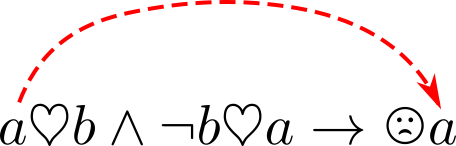
\includegraphics[scale=0.6]{consequent-copy.png}}}
\end{equation}
\uline{These two actions (\textbf{compare} and \textbf{copy}) are hard to do with neural networks}. But they are the essence of variable substitution and the trouble of predicate logic. In other words, it is difficult to accomplish these two actions in one breath with a monolithic end-to-end neural network:\begin{equation}
\vcenter{\hbox{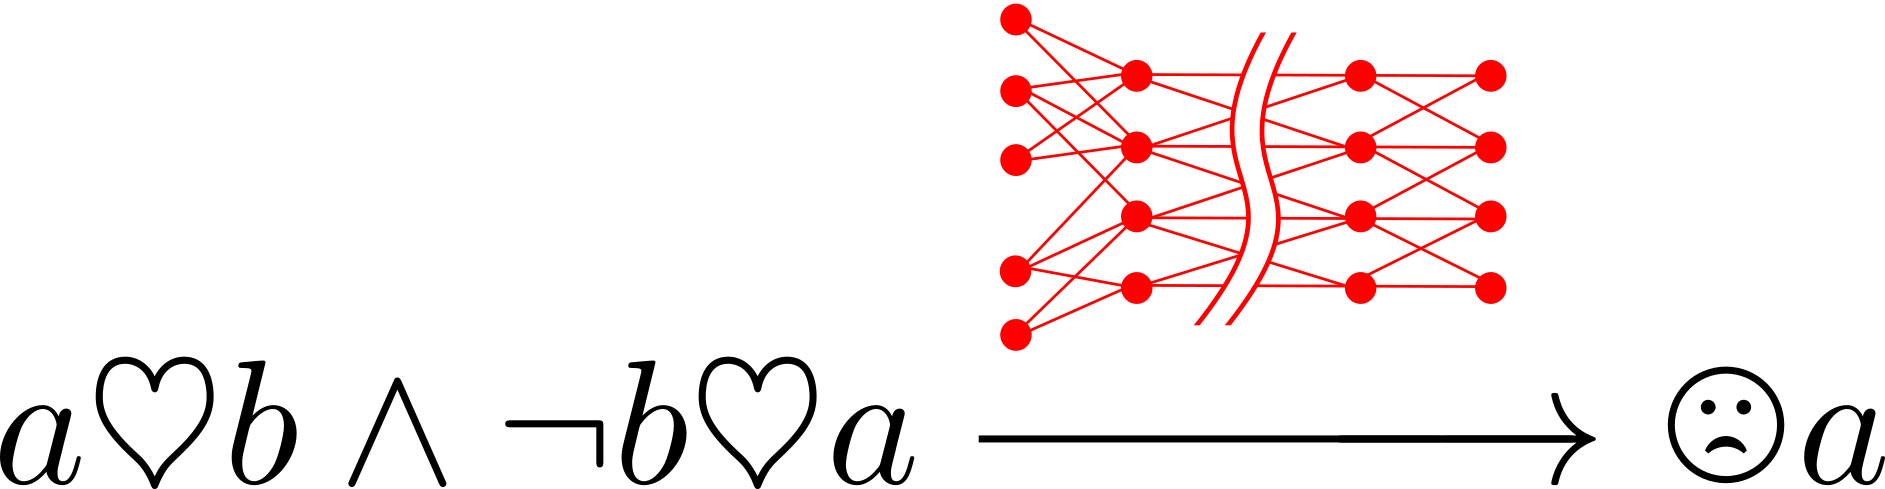
\includegraphics[scale=0.6]{monolithic-NN.png}}}
\end{equation}

First consider the copy problem of \textbf{poster}. For simplicity, assume that the logical variable $z$ corresponds to some component of the input vector $\vec{x}$, such as $x_i$. The purpose of Copy is to copy $x_i$ to the $y_j$ position:\vspace*{10pt}
\begin{equation}
\vec{F}: \; (x_1, ..., {\color{red} x_i} \tikzmark{a}, ... , x_n) \mapsto (y_1, ... , \tikzmark{b} {\color{red} y_j} , ... , y_n)
\begin{tikzpicture}[overlay,remember picture,out=45,in=135,distance=1.1cm]
  \draw[->,red,shorten >=7pt,shorten <=7pt] (a.center) to node [auto, above=2pt] {$id$} (b.center);
\end{tikzpicture}
\end{equation}
This requires the function surface of the neural network to pass through some diagonal lines, as shown below:\begin{equation}
\vcenter{\hbox{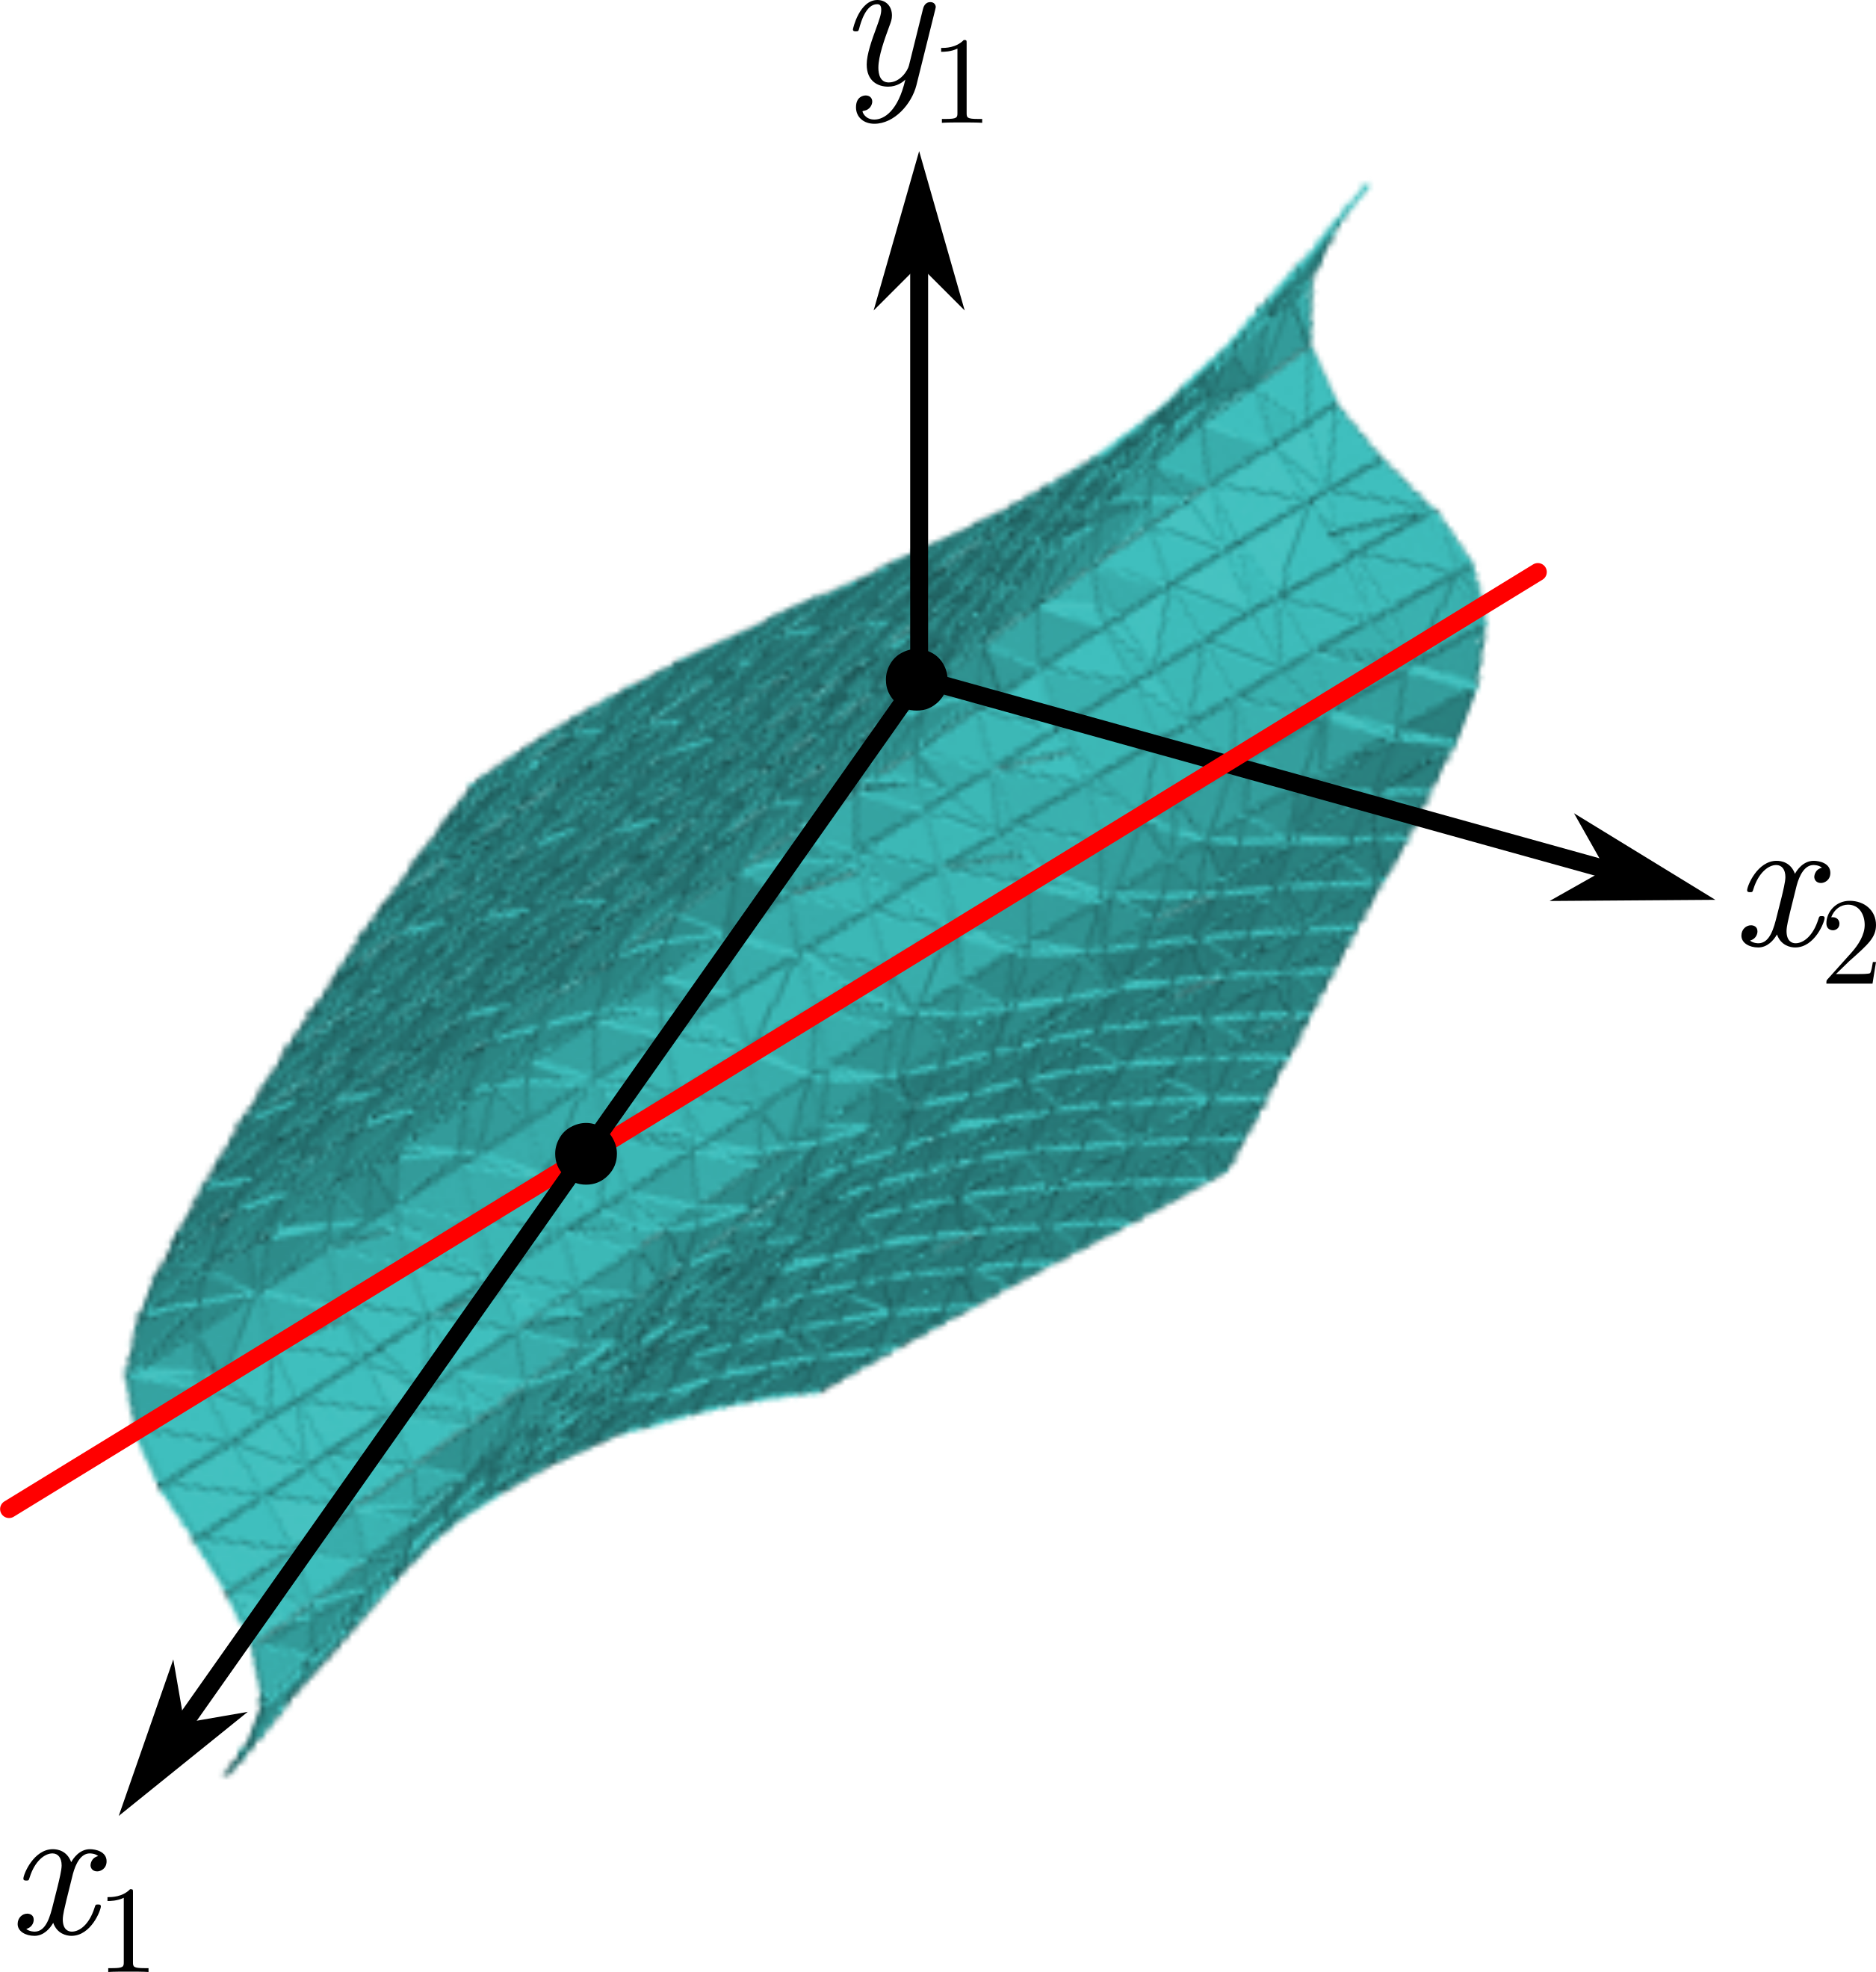
\includegraphics[scale=0.4]{diagonal.png}}}
\end{equation}
The following is a simple copier neural network (ownership weight = 1, other weights = 0 not shown):\begin{equation}
\vcenter{\hbox{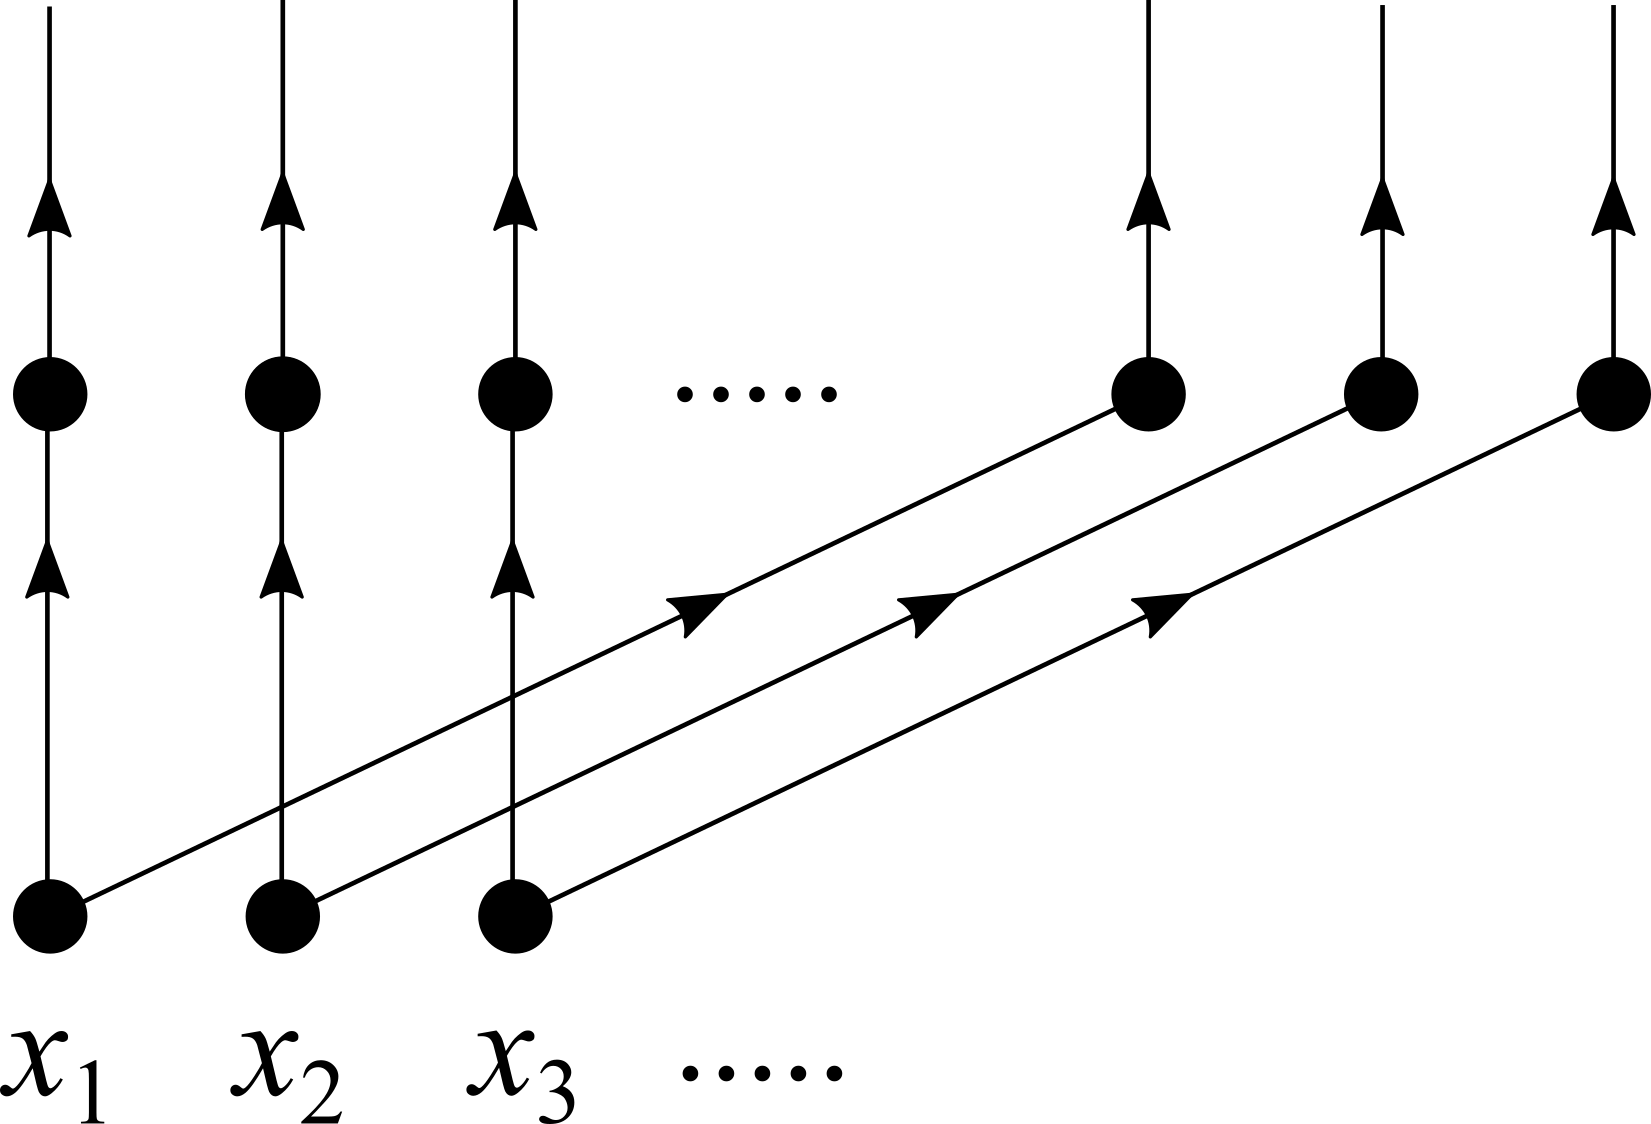
\includegraphics[scale=0.7]{NN-copying.png}}}
\end{equation}
A neural network with input dim = $n$ and output dim = $2 n$, if fully connected, needs to train $2 n^2$ weights. But I haven't had time to test how long it takes to train a multi-layer neural network to learn this action.
Second, consider the establishment of \textbf{frontware}, a viable \textbf{geometric image} is such a \footnote{this is just one of many possible representations, but it seems that any "geometric" form of representations has similar problems. . Unless we consider representations with the characteristics of ``procedural''? The following will discuss .... }:\begin{equation}
\vcenter{\hbox{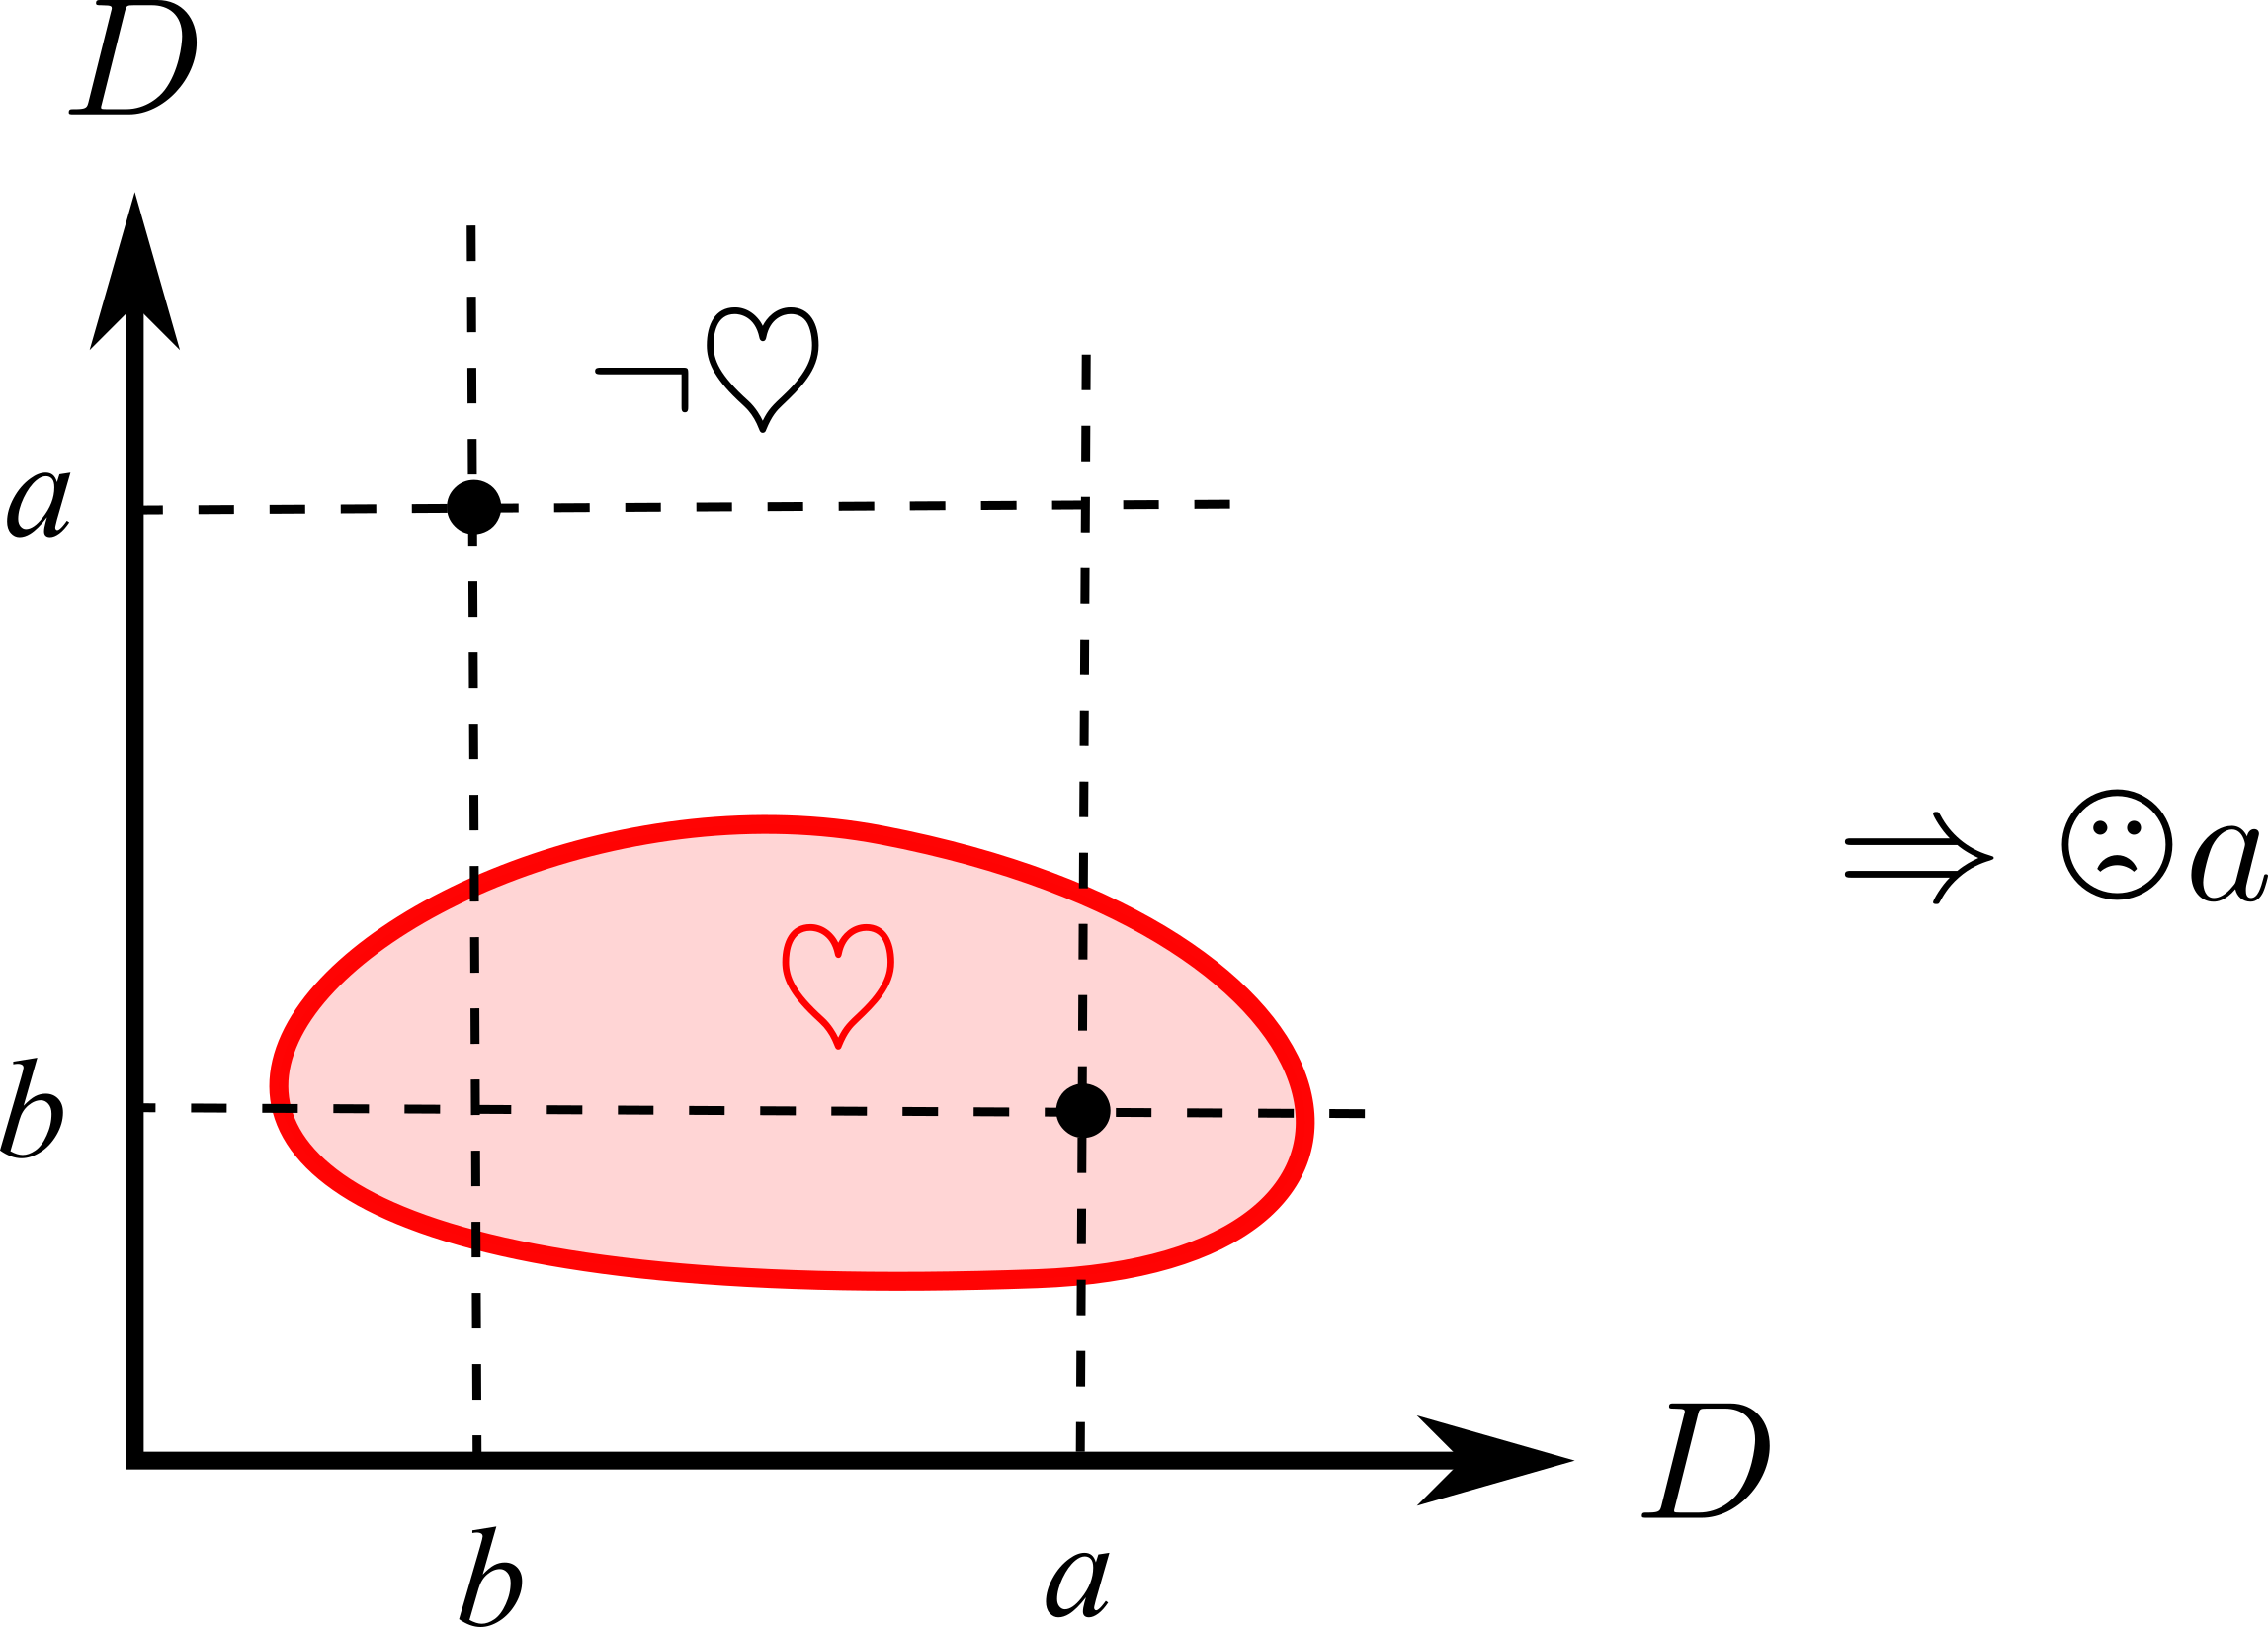
\includegraphics[scale=0.6]{heart-break.png}}}
\end{equation}
$\in$ is easy to solve with a neural network, for example $\heartsuit$ can be defined as a neural network:\begin{equation}
\heartsuit (\vec{x}) = \begin{cases}
0 & \vec{x} \notin \mbox{region}\\
1 & \vec{x} \in \mbox{region}
\end{cases}
\end{equation}
但即使这样,仍然馀下一个 pattern matching (comparison) 问题:
\begin{eqnarray}
\vec{p}_1 = (\tikzmark{a1} \vec{a}, \vec{b} \tikzmark{b1}) &\in& \heartsuit \nonumber \\
&& \nonumber \\
\vec{p}_2 = (\tikzmark{b2} \vec{b}, \vec{a} \tikzmark{a2}) &\in& \neg \heartsuit
\begin{tikzpicture}[overlay,remember picture]
  \draw[-, red, shorten <=20pt, transform canvas={shift={(-3pt,13pt)}}] (a1.center) to (a2.center);
  \draw[-, red, shorten <=20pt, transform canvas={shift={(-6pt,13pt)}}] (a1.center) to (a2.center);
  \draw[-, red, shorten <=20pt, transform canvas={shift={(5pt,13pt)}}] (b1.center) to (b2.center);
  \draw[-, red, shorten <=20pt, transform canvas={shift={(2pt,13pt)}}] (b1.center) to (b2.center);
\end{tikzpicture}
\end{eqnarray}
The following is a simple comparator simulated with the RNN neural network (all = 0 weights are not shown):\begin{equation}
\vcenter{\hbox{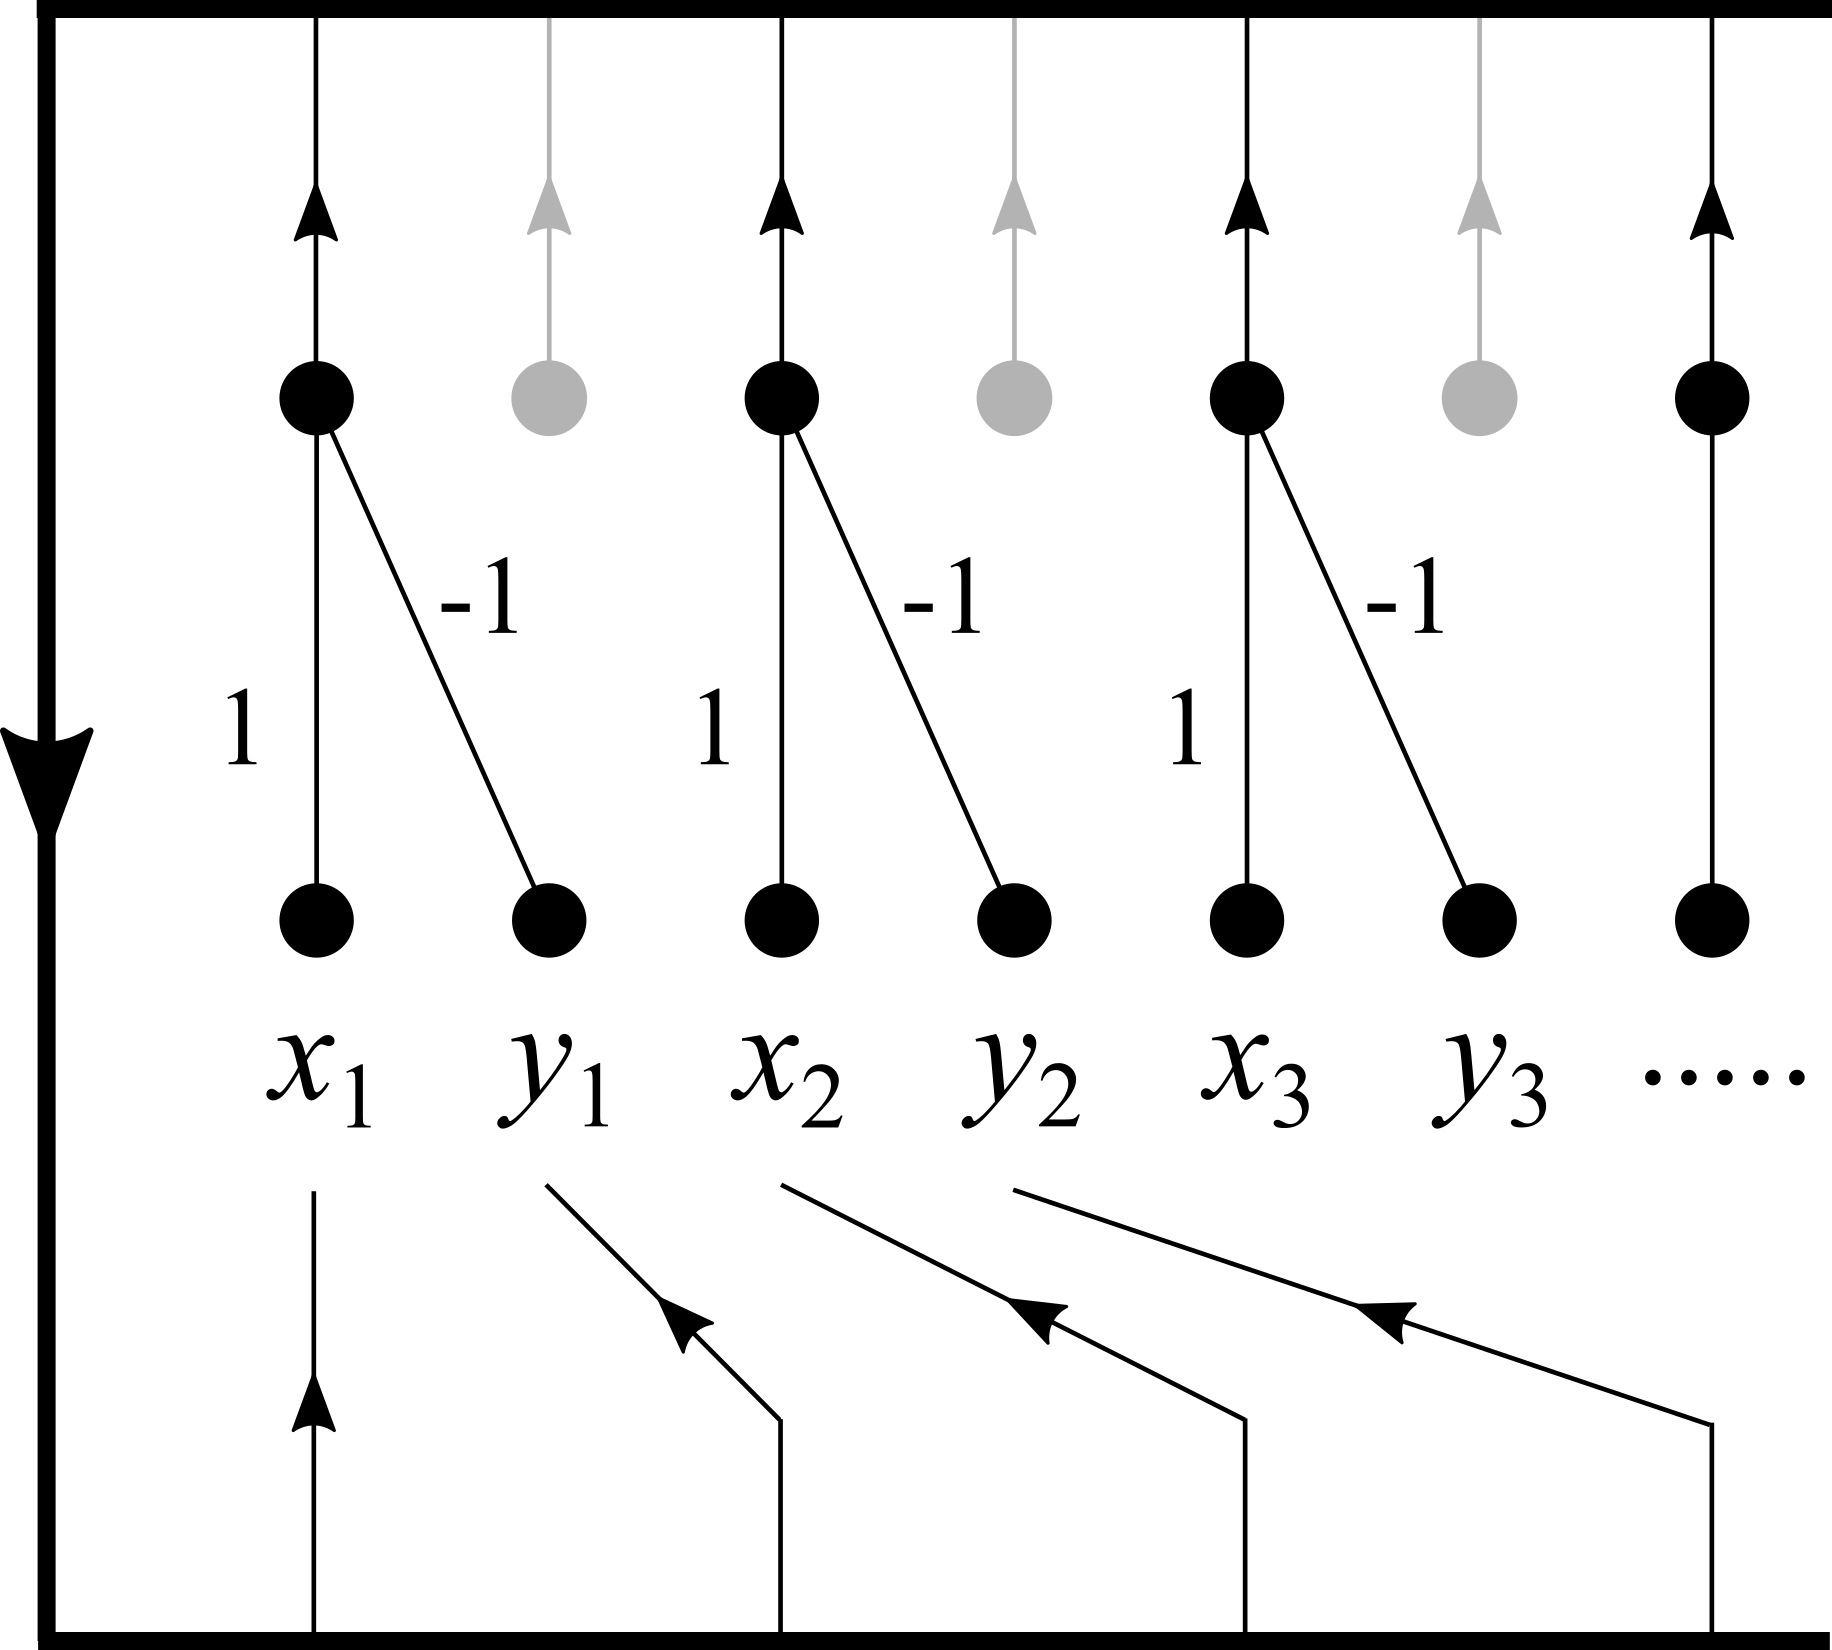
\includegraphics[scale=0.7]{NN-comparator.png}}}
\end{equation}
在 iterate $n$ 次之后,最左边的输出 会是 $\vec{x} \stackrel{?}{=} \vec{y}$ 的真假值。 假设 输入维数是 $2 n$,需要训练 $(2 n)^2$ 个 weights。

Conclusion: Based on the above analysis, it seems not very difficult to simulate copier and comparator with NN, but in fact, these "components" are used in conjunction with short-term memory, and the entire architecture is still unknown.

\subsection{``Distributive'' representations}

% Distributive representation 是针对神经网络而言的,因为神经网络是现时最强的机器学习方法(除了我最近开始提倡使用的 \textbf{基因算法})。

The meaning of \textbf{Distributive representation} is: Suppose there is a vector indicating that the output of the neural network has $n = 10$ granule neurons:\begin{equation}
\vec{x} = (x_1, x_2, .... , x_{10})
\end{equation}
In binary, each $x_i \in \{ 0, 1 \}$, $\vec{x}$ can represent the concept of 10 ``\textbf{one-hot}'' respectively. But if you use distributive representation, these 10 bits can express up to $2^n = 1024$ different states/concepts. But in fact, the conjunctions of one-hot features are not different from distributive representations if they are treated as different states. So, the representation of a neural network can be said to be $\mathbb{R}^n$ vector , or as $n$ coordinates of the $n$-dimensional manifold.
For example, \textit{``John throws ball to Mary''} This image, after processing such as CNN, can get a \textbf{distributed knowledge representation}:\begin{equation}
\vcenter{\hbox{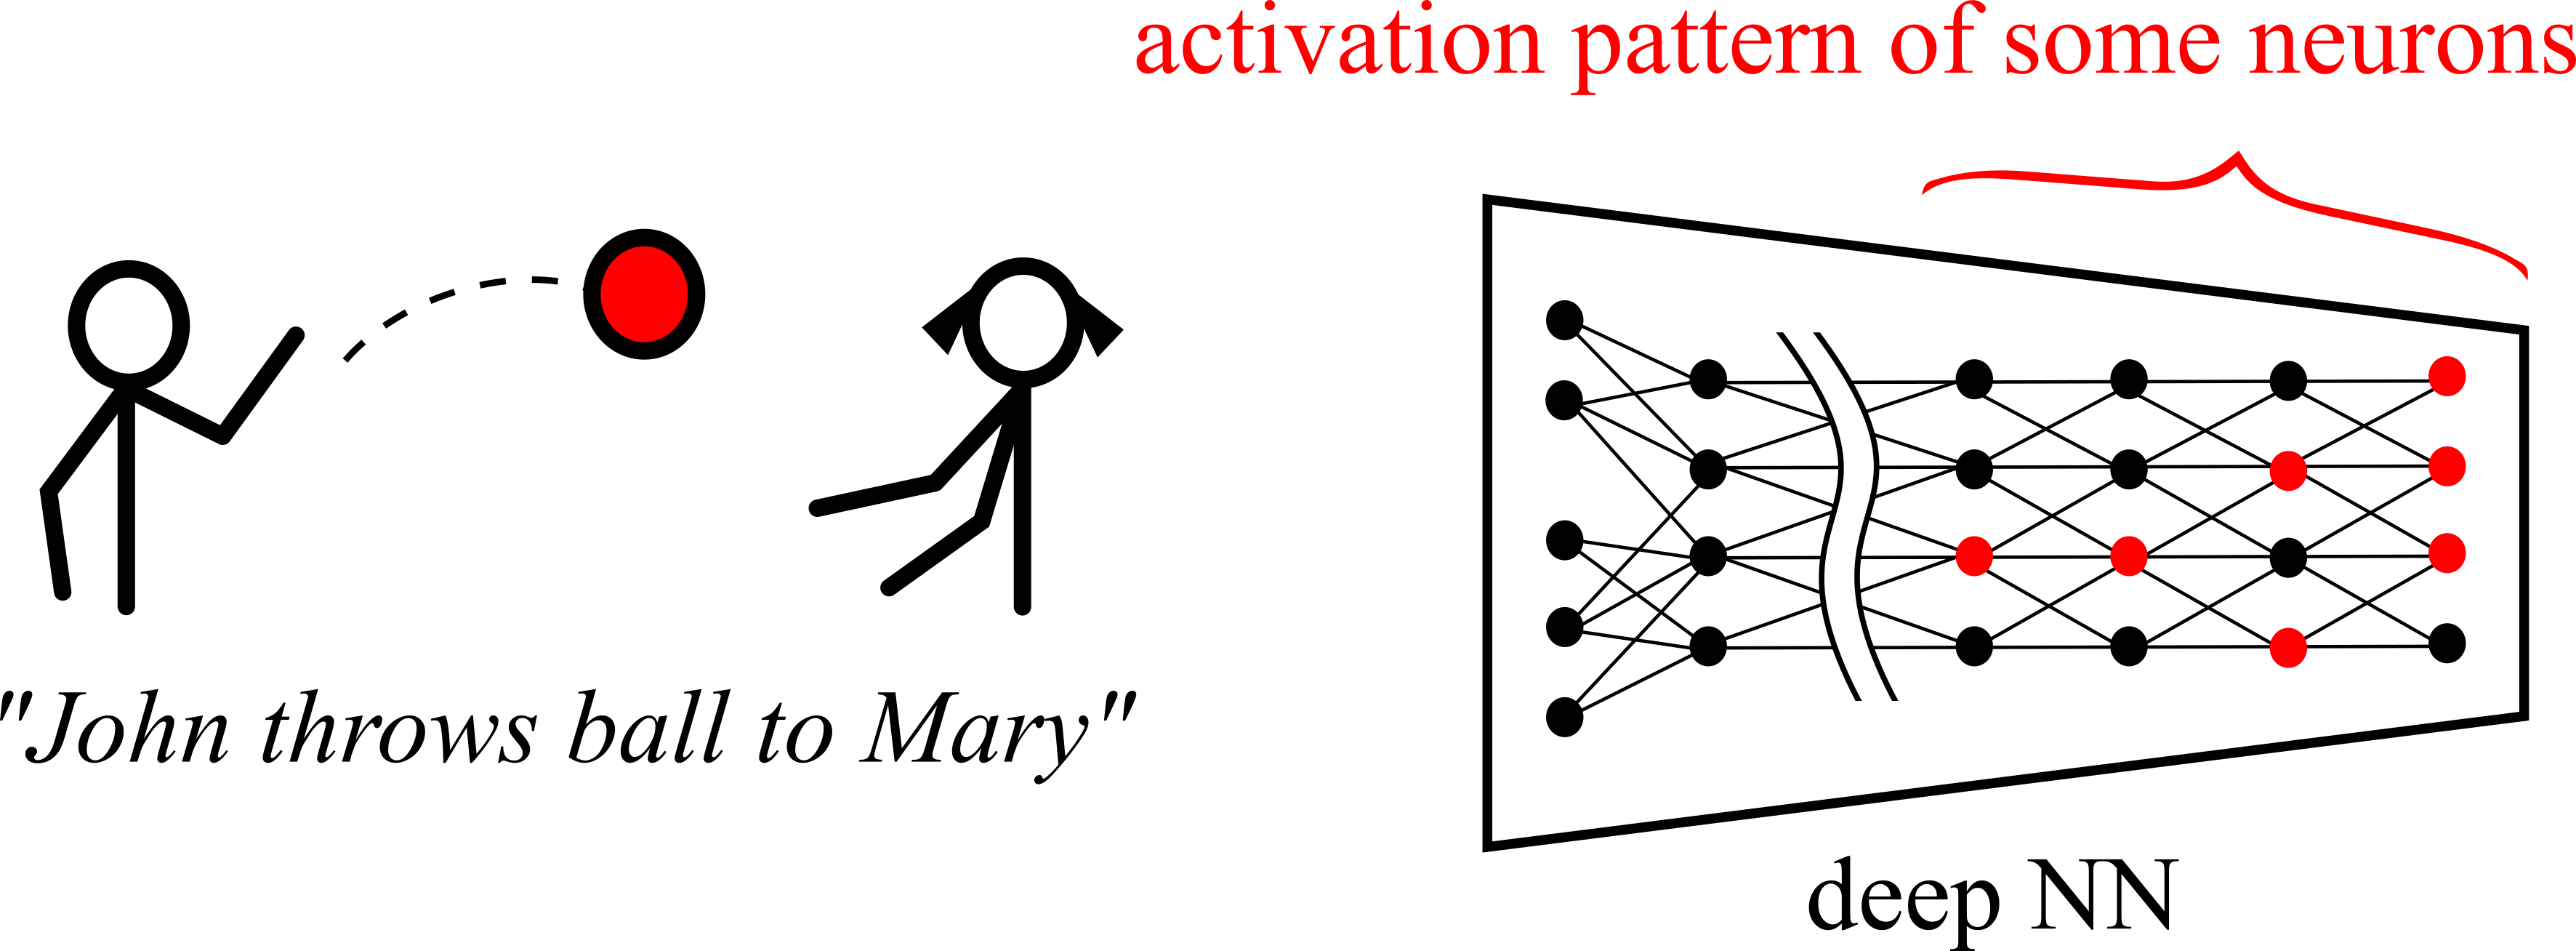
\includegraphics[scale=0.7]{NN-activation-patterns.png}}}
\end{equation}
%注意那些红点不一定是\textbf{最后}那层的输出。  这是我心目中的图像,比较 general,不是指某个特定的 implementation。  重点是: 「美女过马路」是一个 ``\textbf{neat}'' 命题,但在感知过程中,我们会认得很多细节,例如「裙子、高跟鞋、金发、斑马线、路灯」等。  这些特徵 (features) 构成整个 representation,至少我是这样理解 分布式表述 的。
This can be understood as: \uline{a ``neat'' proposition is broken down into a number of small propositions}, for example:\begin{equation}
\mbox{A 掷球给 B} \Longleftrightarrow \left\{
                \begin{array}{l}
                  \mbox{A手臂挥动 } \; \wedge \\
                  \mbox{球离开A的手 } \; \wedge \\
                  \mbox{球在半空飞 } \; \wedge \\
                  ...
                \end{array}
              \right.
\end{equation}
These two sides are \textbf{logically equivalent}. The details of "The ball is red" cannot appear on the right side, because this detail is not left \textbf{implication}. But there can be "the ball is usually round". in other words:\begin{equation}
\boxed{\mbox{``neat'' proposition}} \quad p \Longleftrightarrow \left\{
                \begin{array}{l}
                  q_1 \; \wedge \\
                  q_2 \; \wedge \\
                  ... \; \wedge \\
                  q_n
                \end{array}
              \right.
\quad \boxed{\mbox{distributed propositions}}
\end{equation}

\textit{Conclusion}: Unknown What is the impact of distributed knowledge representation on AI? For the time being, our architectures are equally applicable to distributive and neat logic, except for the increase in the number of propositions and the part of the "visual nerve".
%经典逻辑表述是由 命题 构成的,其实 features 也可以看成是命题,例如「高跟鞋」可以看成是「有一只高跟鞋在这位置」的命题。 逻辑上来说:
%\begin{equation}
%\boxed{\mbox{neat proposition}} \quad p \Leftrightarrow \bigwedge q_i \quad \boxed{\mbox{distributive features}}
%\end{equation}
%有时(例如纯文字输入时),知道的只是一个 neat 命题,例如「美女过马路」,并不知道其他细节(例如「金发」),这时仍然可以有分布式表述,但那些特徵会是比较抽象的。

\subsection{Neural networks lacks short-term memory mechanism}

Consider the image of "White Cat Chasing Black Cat":\begin{equation}
\vcenter{\hbox{
\includegraphics[scale=0.65]{white-cat-chase-black-cat.png}}}
\end{equation}
The concept of "cat" needs to appear \textbf{twice}, but the feature corresponding to "cat" in the neural network is only \textbf{set} (unless there are two duplicate modules that can represent any concept, but it is wasteful) . In other words, the current CNN does not have the ability to "traverse" the field of view; \uline{it cannot distinguish and describe the }\textbf{\uline{relationship}} between objects.
It's hard to imagine how a ``monolithic'' neural module (such as feed-forward NN or RNN) can do this. It seems necessary to express the proposition as a series of concepts of \textbf{time sequence}, some kind of \textbf{short-term memory} (\textbf{STM}, short-term memory).
I was a little surprised to find that the current neural network does not have the mechanism of \textbf{short-term memory}, and "short-term" means that the time-scale is shorter than the time when the weights change. For example, I tell you a string of numbers (such as a phone number), you can remember it in the brain, but this mechanism seems to have no research in the current artificial neural network, perhaps some models in computational neuroscience, but for the time being I don't know. Without such an STM, it is difficult to simulate symbolic logic. In other words, strong artificial intelligence cannot be achieved.
For example, using NN to implement a \textbf{dynamic memory}, when it receives a new element, it will \textbf{compare} to other elements in the memory, and it has the \textbf{copy} function. For example, the following time series mechanism like "Rotating Trojan" (each $\NewSym{distributive-vector.png}$ represents a distributive vector):\begin{equation}
\vcenter{\hbox{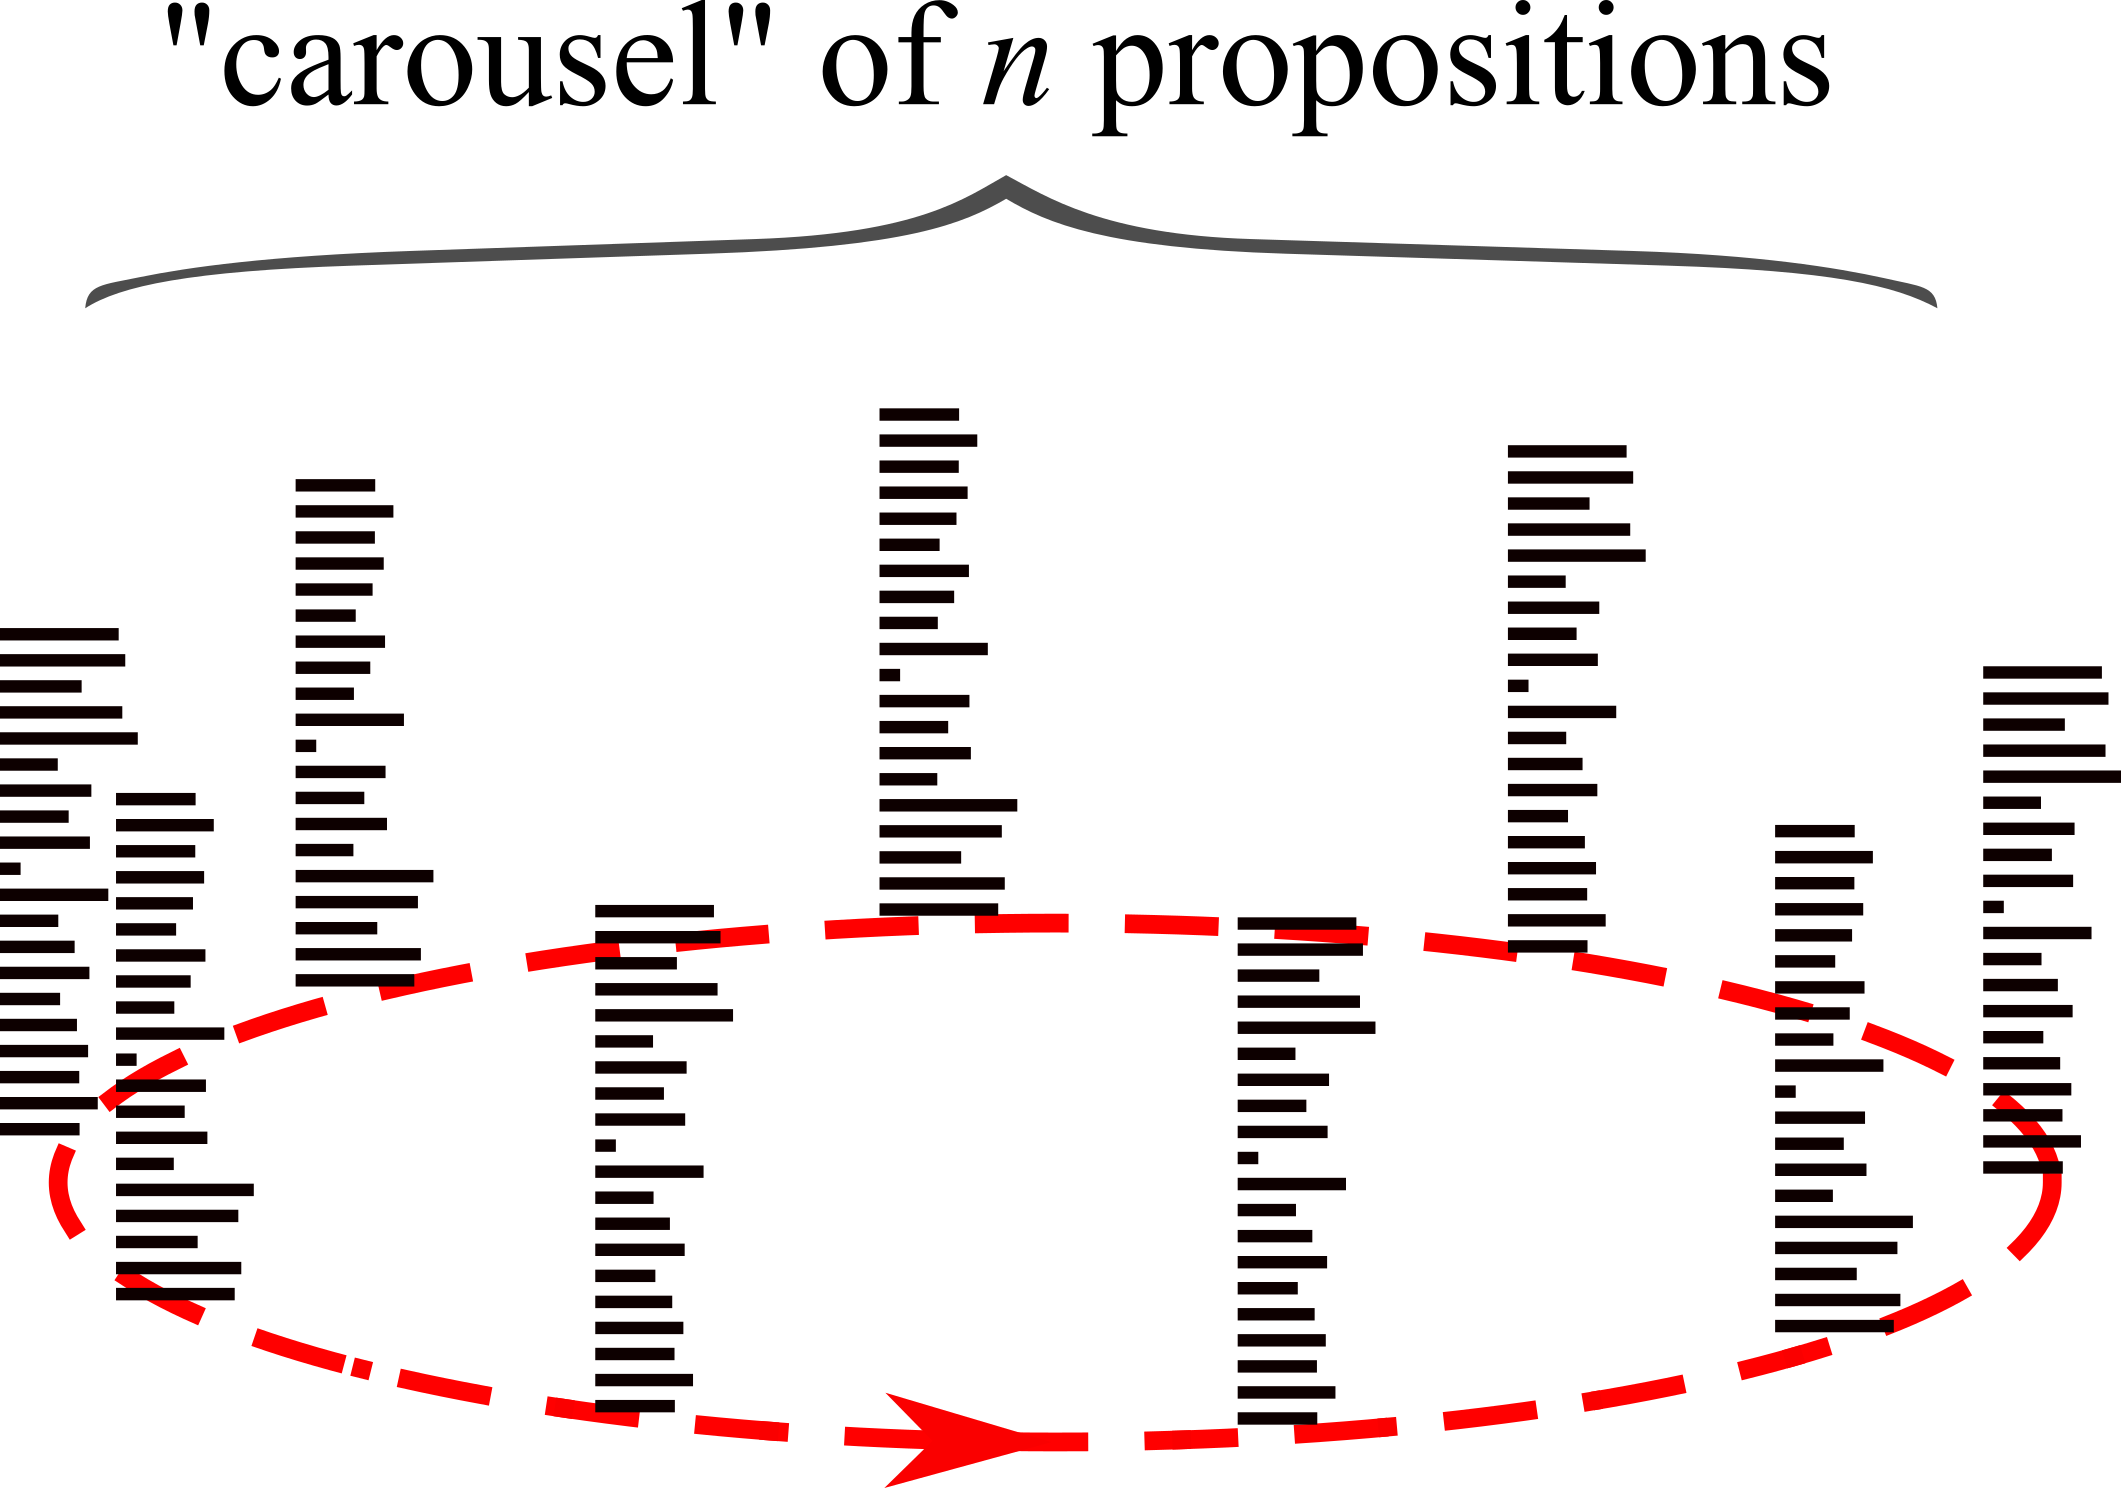
\includegraphics[scale=0.7]{carousel-of-vectors.png}}}
\end{equation}
In short, it's obviously cumbersome to simulate STM purely with NN.
%\begin{tcolorbox}[breakable, colback=yellow]
%用神经网络解决强人工智能的最大障碍是 从命题逻辑到一阶逻辑的\textbf{跃升},特别是 substitution 运算,需要有 short-term memory 机制
% The bottleneck of strong AI is the \textbf{learning algorithm}'s speed, and the most crucial obstruction is the \textbf{lifting} from propositional to first-order logic.
%\end{tcolorbox}

\subsection{Graph neural networks}
\label{graph-NN}

\begin{tcolorbox}[ams equation, colback=yellow, colframe=white]
\mbox{用 graph 做记忆体(包括短期和长期记忆)}
\end{tcolorbox}
When adding a new memory unit, the same nodes will be matched into one. In other words, the matching step is solved by the traditional symbolic method, and the problem is left to the neural network.\begin{eqnarray}
\mbox{model } \mathcal{M} &=& \mbox{graph} \nonumber \\
\mbox{rewriter} &=& \mbox{deep NN = graph neural network}
\end{eqnarray}

Many thanks to the graph network paper \parencite{Battaglia2018} published by Google / DeepMind in June 2018, Peter Battaglia and 26 collaborators surveyed the development of graph network. The graph network they proposed is closer to some physical systems such as springs and spheres, rather than the first-order model, but essentially the same.
Usually the model is too large, you need to use the attention mechanism to select a fragment of it, and then ``present'' to handle the neural network:\begin{equation}
\vcenter{\hbox{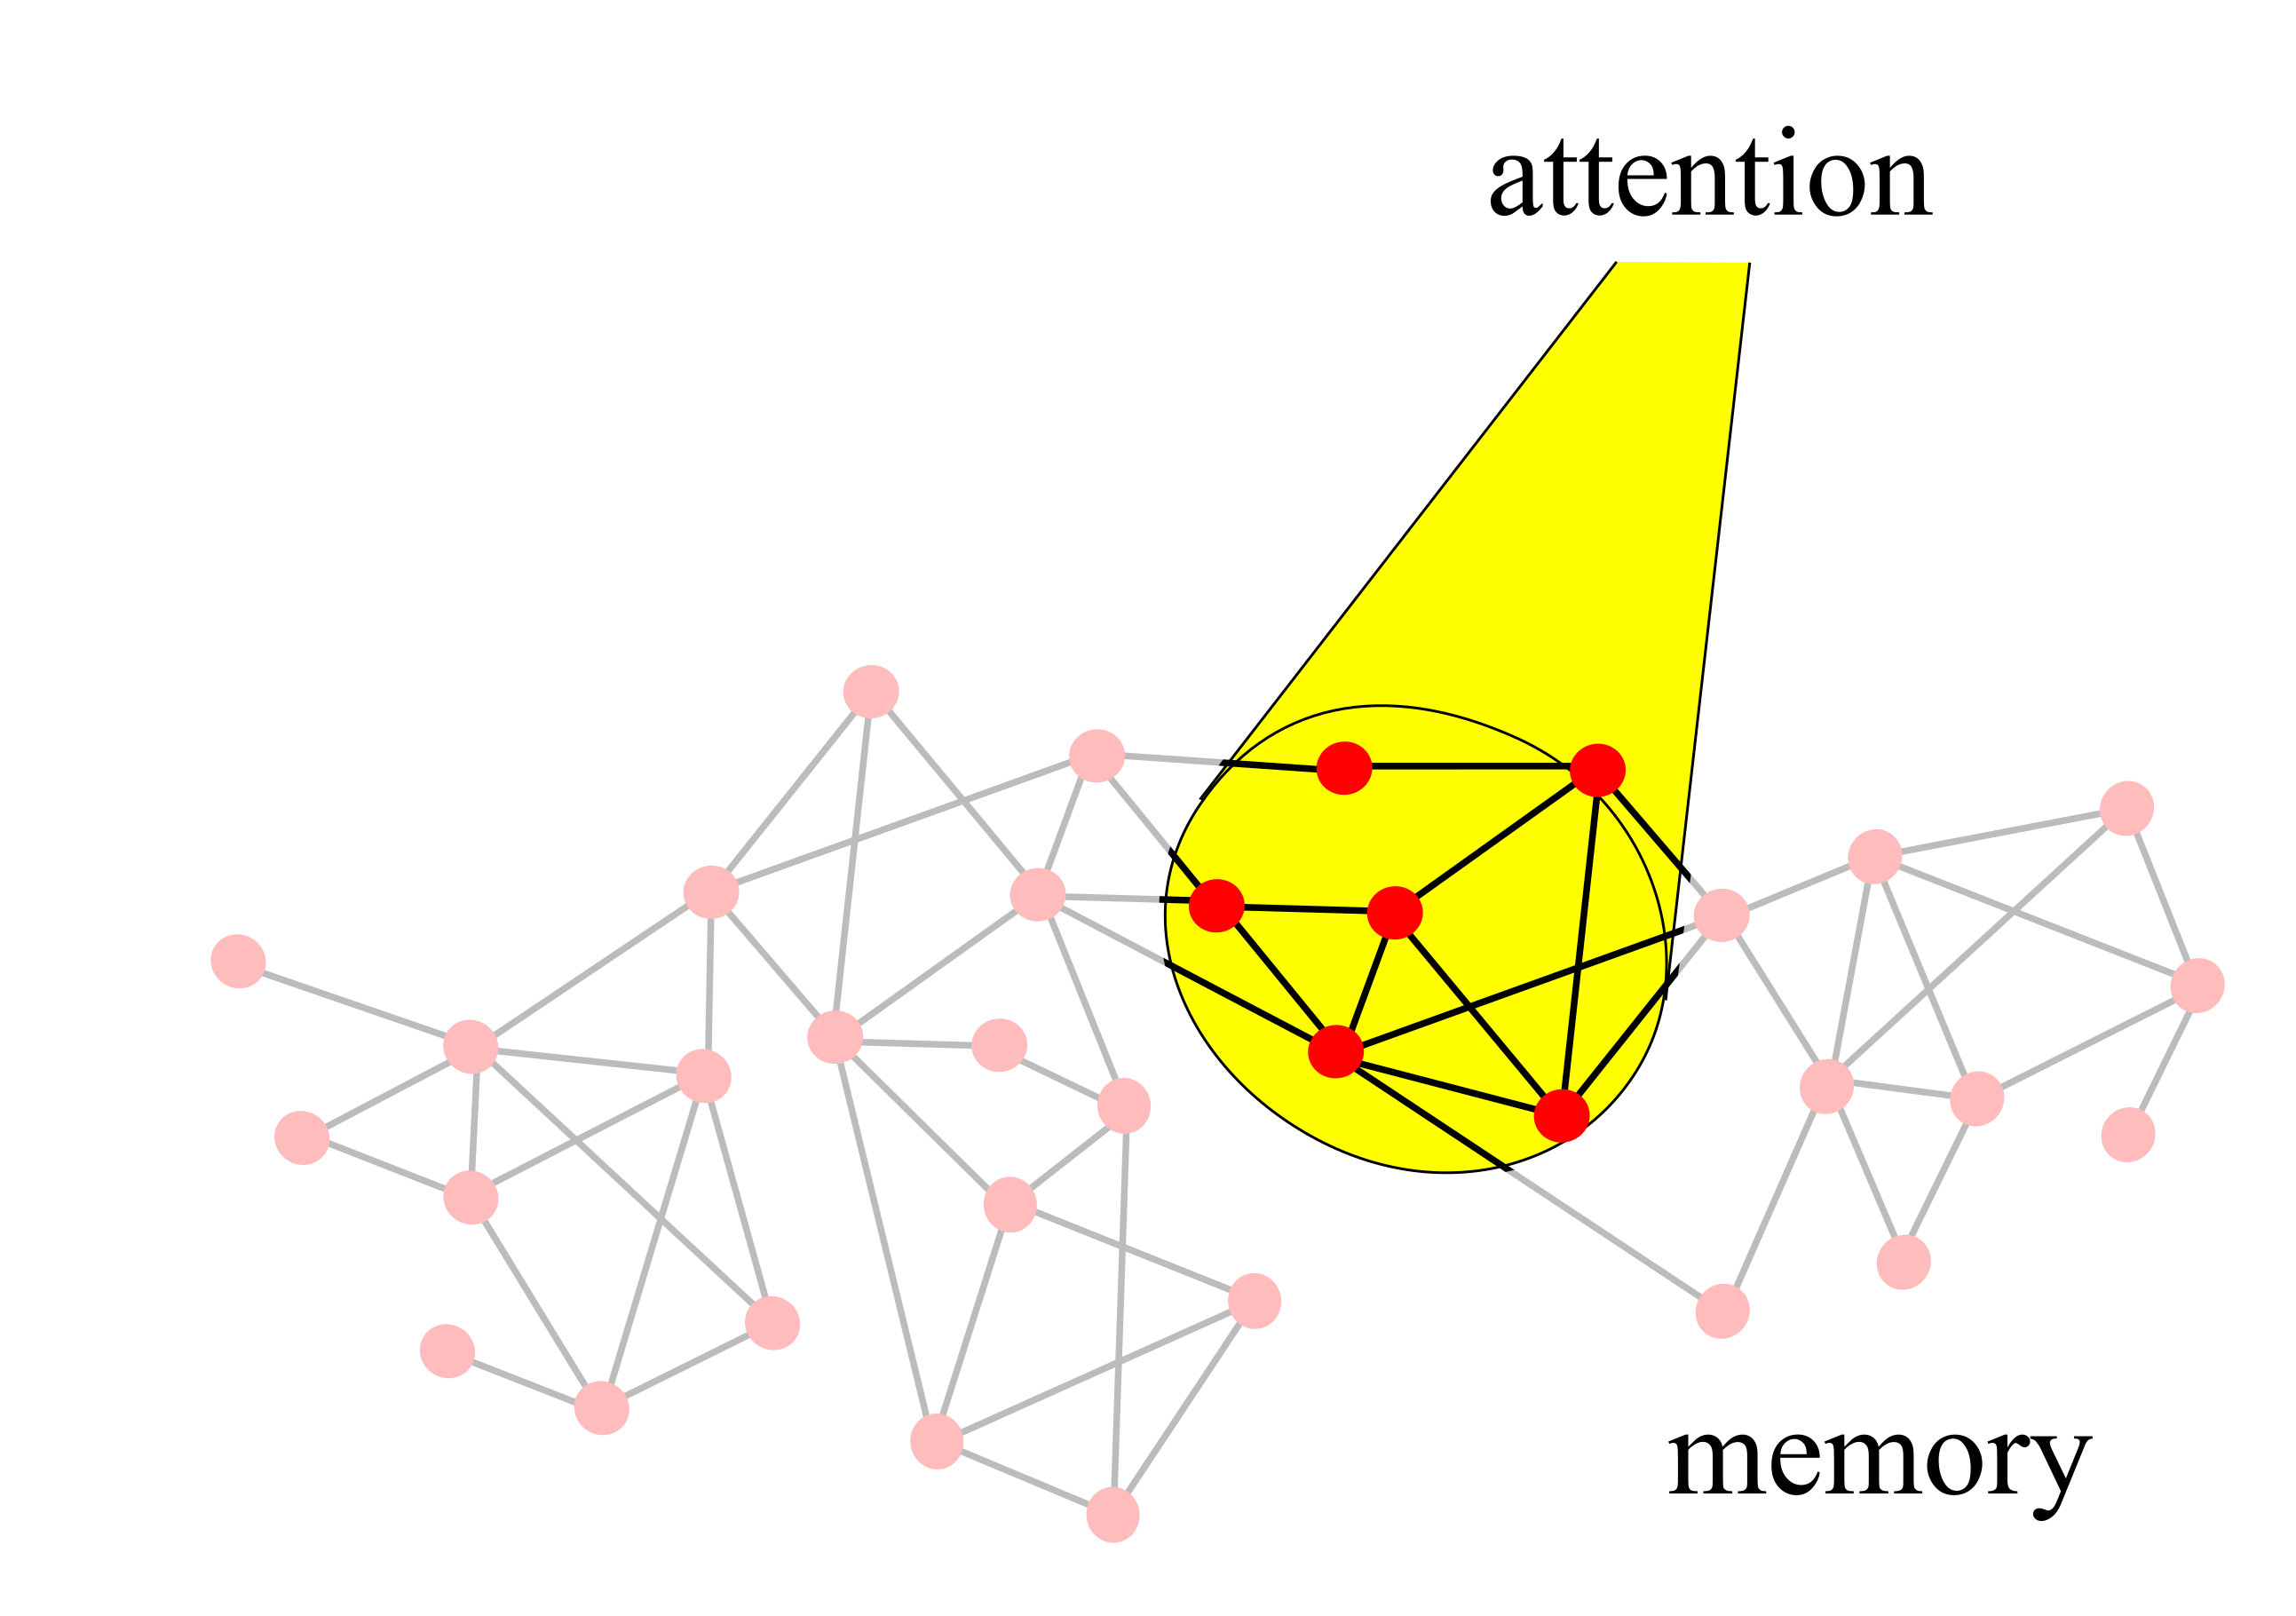
\includegraphics[scale=0.7]{attentional-mechanism.png}}}
\end{equation}
This attention mechanism is somewhat different from the attention in the current deep learning or in the specific details, but basically the same concept.
The neural network input $\vec{x}$ requires an embedding like this:\begin{equation}
\boxed{\mbox{graph}} \quad
\begin{tikzcd}[column sep = large]
\NewSym[1.5]{../graph-symbol.png} \ar[r, hookrightarrow, "\mbox{embed}"] & (x_1, ..., x_m) 
\end{tikzcd}
\quad \boxed{\mbox{vector}}
\end{equation}
But graph is not a "linear" structure \footnote{linear means symbolic form, for example, tree can be represented as a linear line}, it seems quite difficult to represent the graph structure as a vector (this may be the delay of the graph neural networks) There are reasons for the breakthrough).
\begin{tcolorbox}[breakable, parbox=false]
There is \textbf{quiver representations} in mathematical representation, which turns vertex into vector space and edge becomes linear transformation between vector spaces. For example:\begin{equation}
\begin{tikzcd}[column sep = large]
\mbox{John} \arrow[r, bend left, "\heartsuit"] & \arrow[l, bend left, swap, "\neg \heartsuit"] \mbox{Mary}
\end{tikzcd}
\quad \Longrightarrow \quad
\begin{tikzcd}[column sep = large]
V_1 \arrow[r, bend left, "M_1"] & \arrow[l, bend left, "M_2"] V_2
\end{tikzcd}
\end{equation}
Where $V_1, V_2$ is the vector space, $M_1, M_2 \in GL(\mathbb{R})$ is the matrix. But this is still not a vector.
Under the \textbf{base transform} of the vector space $V_i$, the two matrices $M$ may be the same linear transform. Therefore, you need to consider their \textbf{invariance}, which is moduli. Representation is concerned with breaking down various $M$ \uline{ into irreducible components}. The Dynkin diagrams that appear in this decomposition are the same as those found in the Lie algebra classification. But if the quiver is not a Dynkin or some extension, then the quiver is ``wild'' and it's hard to break. Even a simple quiver can be a wild type.
Each quiver defines a path algebra whose elements are the path in the quiver, in other words the logical \textbf{relationship} and its composition. For the time being, I don't know what quiver representations are for in AI.\end{tcolorbox}

The overall operation is like this:\begin{equation}
\vcenter{\hbox{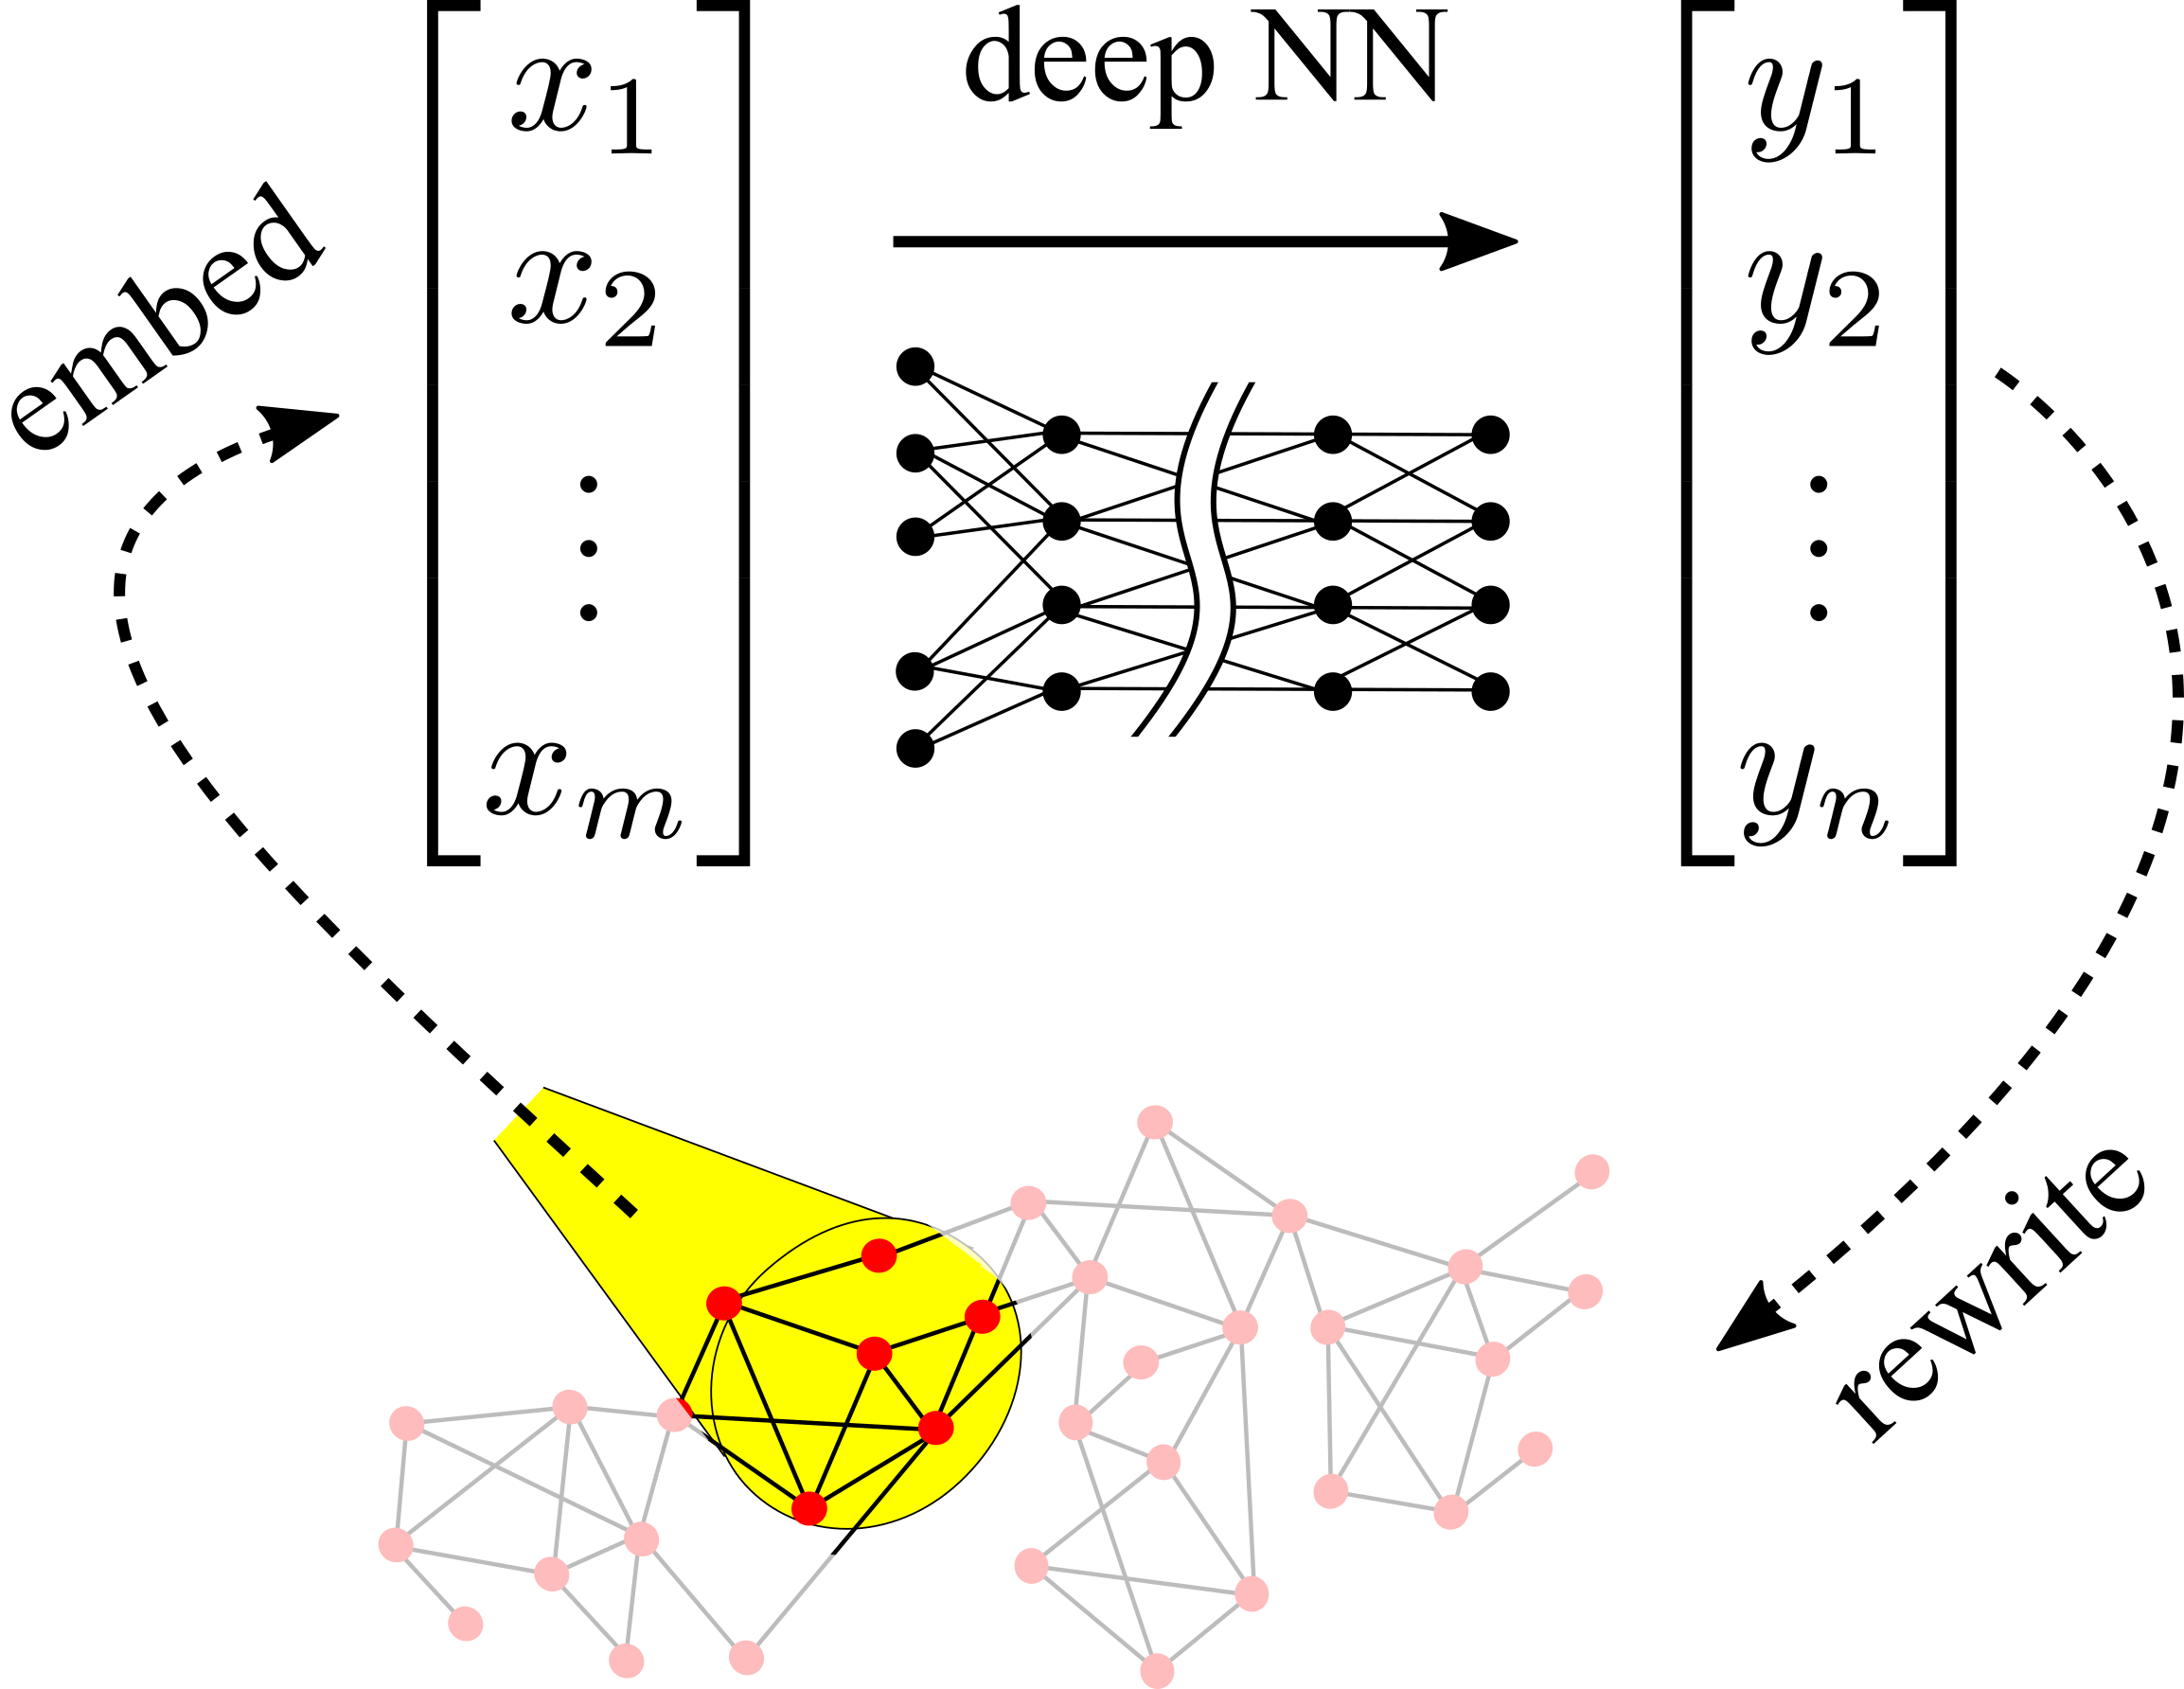
\includegraphics[scale=0.6]{graph-NN-rewriting.png}}}
\end{equation}
This deep NN can be either CNN or RNN because they are currently very successful in natural language understanding/translation, but they deal with linear sequence inputs. Or you can split the memory sub-graph into linear elements (that is, individual relationships/propositions), and you can't use global variable references (in other words, variable matching has been done). Then the variable copying output by NN is also externally processed. In other words, in combination with NN and \textbf{graph rewriting} in the ``hybrid'' way. I still haven't seen a good solution for the embedding details in the picture, but DeepMind / Google's research is very close.
Note: Although the parameter space $\Theta \in \mathbb{R}^N$ of NN is \textbf{continuous}, the rewriting rules it learns are \textbf{discrete} because graph itself is a discrete structure. .
Add a point: attention mechanism to traverse memory graph, in other words a graph search algorithm, this part can be combined with NN into the same module (there are many RNN architectures now).
\begin{center}
\rule{0.4\textwidth}{.6pt}
\end{center}
馀下 2 节是一些 数学 背景知识....

\section{Categorical semantics}
\label{Categorical-semantics}

Categorical semantics is a model theory expressed in category theory.
\book{以下内容主要来自 \parencite{Caramello2018} 这本新书的第一章。  更经典的参考书是 \parencite{Goldblatt2006}.  范畴论最好的入门书当然是「中学生也能看懂的」\textit{Conceptual mathematics} \parencite{Lawvere1997} 还有 \parencite{Lawvere2003}.}

Different logics can be defined by \textbf{proof theory} (which studies \textit{syntactic} rules of deduction):\begin{equation}
\begin{tabular}{|l|l|}
\hline
algebraic logic & no additional rules\\
\hline
Horn logic & finite $\wedge$ \\
\hline
regular logic & finite $\wedge$, $\exists$, Frobenius axiom\\
\hline
coherent logic & finite $\wedge$ and $\vee$, $\exists$,\\
				& distributive axiom, \\
				& Frobenius axiom \\
\hline
geometric logic & finite $\wedge$, infinitary $\vee$, $\exists$,\\
				& infinitary distribution axiom,\\
				& Frobenius axiom \\
\hline
first-order intuitionistic logic & all finitary rules \\
				& except law of excluded middle\\
\hline
first-order classical logic & all finitary rules \\
\hline
\end{tabular}
\end{equation}

For example, \textbf{algebraic theory} means: It has only one relation $=$, and all axioms are of the form $s = t$.
There are also examples of these deduction rules:\begin{equation}
\boxed{\wedge \mbox{ rule}}	\quad \frac{\Phi \vdash \Psi, \; \Phi \vdash \Chi}{\Phi \vdash (\Psi \wedge \Chi)}
\end{equation}
\vspace*{-5pt}
\begin{equation}
\boxed{\exists \mbox{ double rule}}	\quad \Dfrac{\Phi \vdash_{\vec{x}, y} \Psi}{\exists y \, \Phi \vdash_{\vec{x}} \Psi}
\end{equation}
\begin{equation}
\boxed{\mbox{Frobenius axiom}}	\quad \Phi \wedge \exists y \, \Psi \vdash_{\vec{x}} \exists y \, (\Phi \wedge \Psi)
\end{equation}

Tarski's model theory "corresponds" the first-order syntax to the \textbf{structure} of the set theory. As a result, different logical syntaxes correspond to different structural categories:\begin{equation}
\begin{tabular}{|l|l|}
\hline
categories with finite products & algebraic logic \\
\hline
Cartesian categories			& Cartesian logic \\
\hline
regular categories				& regular logic \\
\hline
coherent categories				& coherent logic \\
\hline
geometric categories			& geometric logic \\
\hline
Heyting categories				& first-order intuitionistic logic \\
\hline
Boolean coherent categories		& first-order classical logic \\
\hline
\end{tabular}
\end{equation}

``Geometric'' logic means \textbf{geometric morphisms}, which can be roughly understood as a mapping between two topois, similar to \textbf{continuous maps} between topological spaces.
\uline{Topos can be understood as a generalization of set theory under the influence of category theory}. Each elementary topos\footnote{Elementary is the meaning of "element" in the collection} There is a \textbf{sub-object classifier} $\Omega$. $\Omega$ is a special object, such as $\{ \top, \ Bot \}$, for \textbf{true and false} binary. Use $\Omega$ to define sub-objects, which is the concept of \textbf{subset} in set theory. For example, ``Love'' is a \textbf{relationship} within $D \times D$, and $D$ is a collection of all "people." You can think of $D \times D$ as full relation, then $\mbox{Love} \subset D \times D$ is its \textbf{subset}. In other words, this is why elementary topos can be used as a \textbf{model} for relational algebra or first-order logic. (see \parencite{Goldblatt2006})
"\textit{Lawvere and Tierney's elementary topoi theory \footnote{around 1960-70} is the most important event in the history of categorical algebra..... It's not just that they prove these things, but that they dare to believe this. It is possible}"--- Peter Freyd.
Some history: Around 1963, the concept of topos came independently from several different sources: Alexander Grothendieck's sheaf theory in algebraic geometry, and F William Lawvere's restatement of set theory with category theory, and Paul Cohen's forcing Theory (the latter is used to solve the \textbf{continuity hypothesis}). Sheaf means: Objects defined on some open sets $V_i$, they are consistent on the overlap $V_i \cap V_j$, which can be ``collate''. The situation is like some charts in differential geometry. . After World War II, Leray, then Cartan, defined sheaf using the open sets method. Later Lazard defined sheaf with \'{e}tale, which is the main motivation for the topos theory. For example, a pre-sheaf on a category $\mathcal{A}$ can be defined as a \textbf{functor}:\begin{equation}
\widehat{\mathcal{A}}: \mathcal{A}^{\mathrm{op}} \rightarrow \mathbf{Set}
\end{equation}
That is, a "layer" set-valued function on the category $\mathcal{A}$. It is ``functor'' so it handles those collating. This functor is contravarient so there is $\mathrm{op}$. Grothendieck Applying sheaf to topology (cohomology), then Jean-Pierre Serre found that it can also be used in algebraic geometry. They and other collaborators wrote the 1623-page masterpiece "SGA IV", which greatly influenced the development of algebraic geometry, resulting in In 1974 Deligne solved the Weyl conjecture. But I am not familiar with algebraic geometry for the time being, so it is not clear what Grothendieck did.... See the book \parencite{MacLane1992} for details.
In the topology space, the complement of an open set $U$ is closed and not necessarily open, so if it is confined within the open sets, the ``negation'' of $U$ should be defined as ``the interior of its complement' '. This causes $U$'s "\textbf{double negative}" not necessarily equal to $U$, in other words, \uline{the algebra of open sets follows \textbf{intuitionistic logic}}, such an algebra is called a \textbf{Heyting algebra}. (cf. ibid.)
There are two kinds of morphisms between Topoi: \textbf{geometric morphisms} and \textbf{logical functors}. The former maintains "geometry", the latter maintains a logical type theory, so there is a definition of \textbf{elementary topos}. The latter is characterized by its \textbf{sub-object classifier} $\Omega$.
以下是根据 \parencite{Caramello2018} Ch.1 整理出来的一张关系图,但我暂时还不太熟悉范畴论的概念,所以也不完全理解: 
\begin{equation}
\vcenter{\hbox{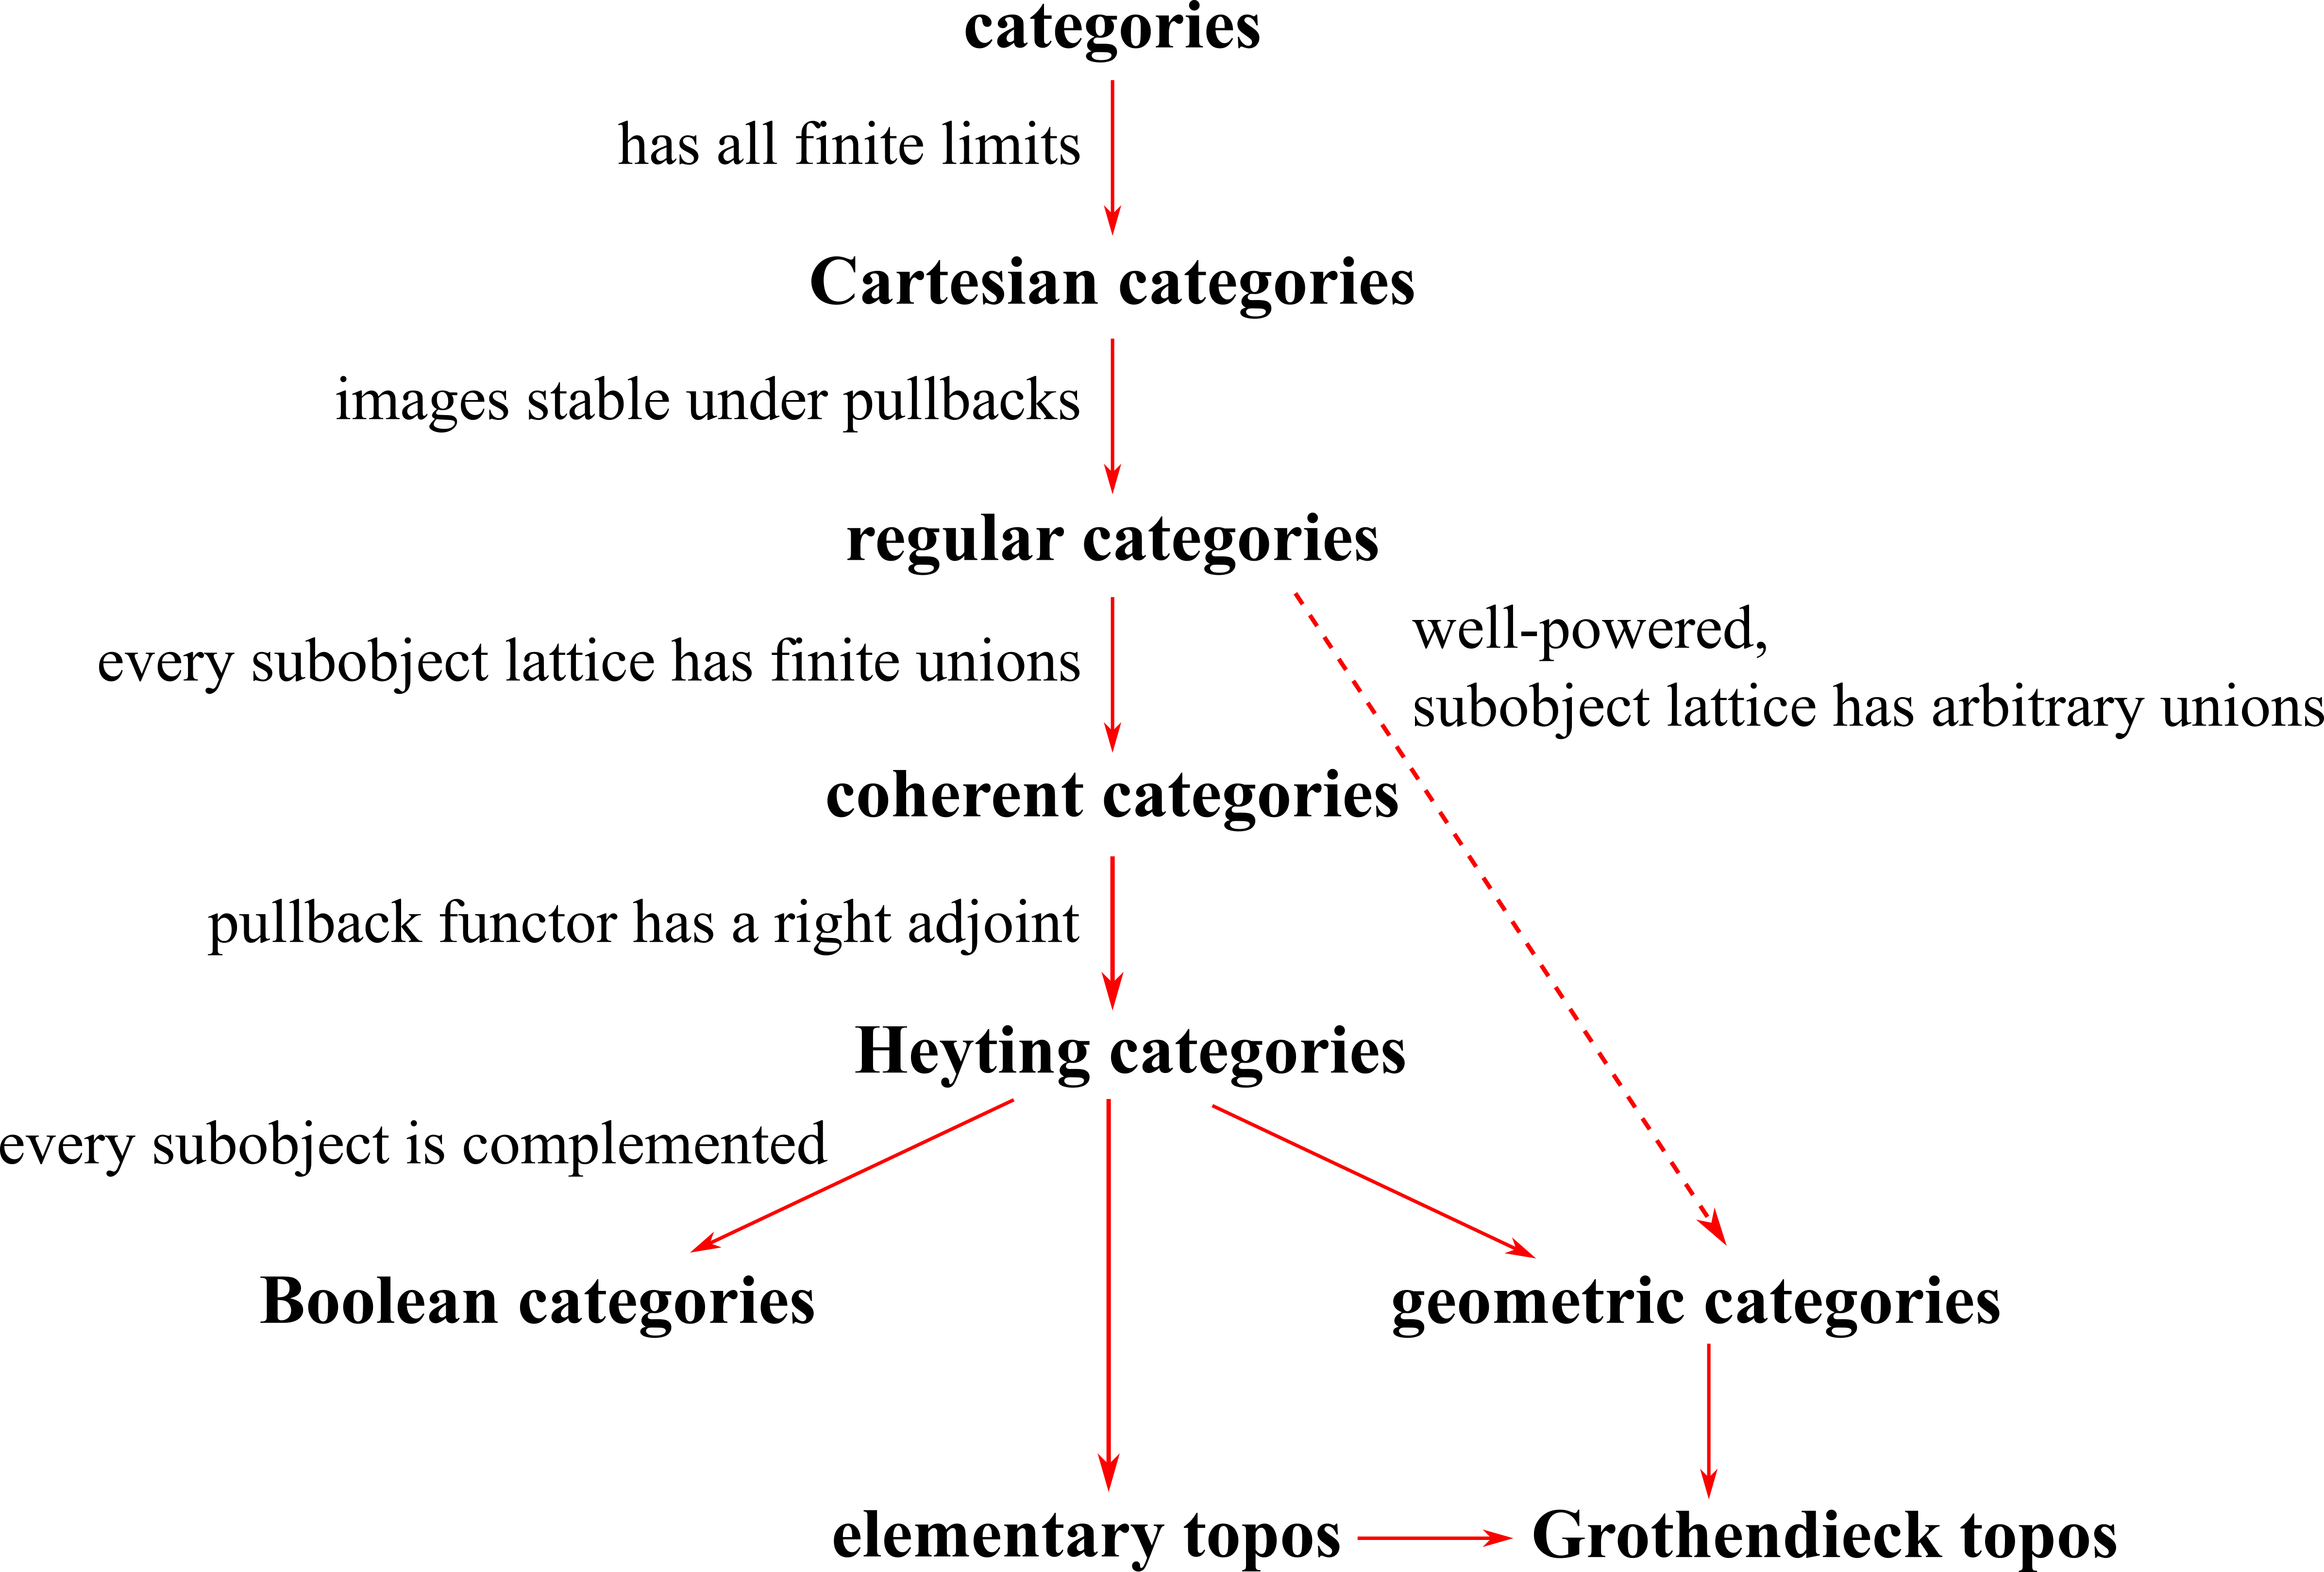
\includegraphics[scale=0.7]{logical-categories.png}}}
\end{equation}

\section{Domain theory}

Both $\lambda$-calculus and combinatory logic can express any form of \textbf{function}. If the domain of the whole function is $D$ and the number of functions by $D \rightarrow D$ is $|D^D|$, $|D^D|$ must be greater than $ according to Cantor's theorem of set theory. |D|$, even if $D$ is infinite, it is still true. In other words, $\lambda$-calculus and combinatory logic are unlikely to have models. This conclusion is very disturbing. But in 1971, the problem was solved by Dana Scott and C Strachey, creating \textbf{domain theory}.
\book{以下内容主要来自 \parencite{Vickers1989},是一本很易懂的书,还有更新和更详尽的 \parencite{Goubault-Larrecq2013}.}

Scott's solution is to give domain $D$ \uline{endow with a \textbf{Scott topology} and then only consider $D \rightarrow D$'s }\textbf{\uline{continuous function}}. The latter is a small number, so it avoids Cantor's theory.
..... 【未完待续】 $\NewSym{../UnderConst.png}$

\printbibliography 

\end{document}
